
\chapter{Entwurf}
\section{Systementwurf}
\subsection{Generelles Data Fetching} \label{data-fetching}
Dieses Abschnitt baut auf das Kapitel \ref{oauth2-strat} auf.
\begin{figure}[!ht]
  \centering
  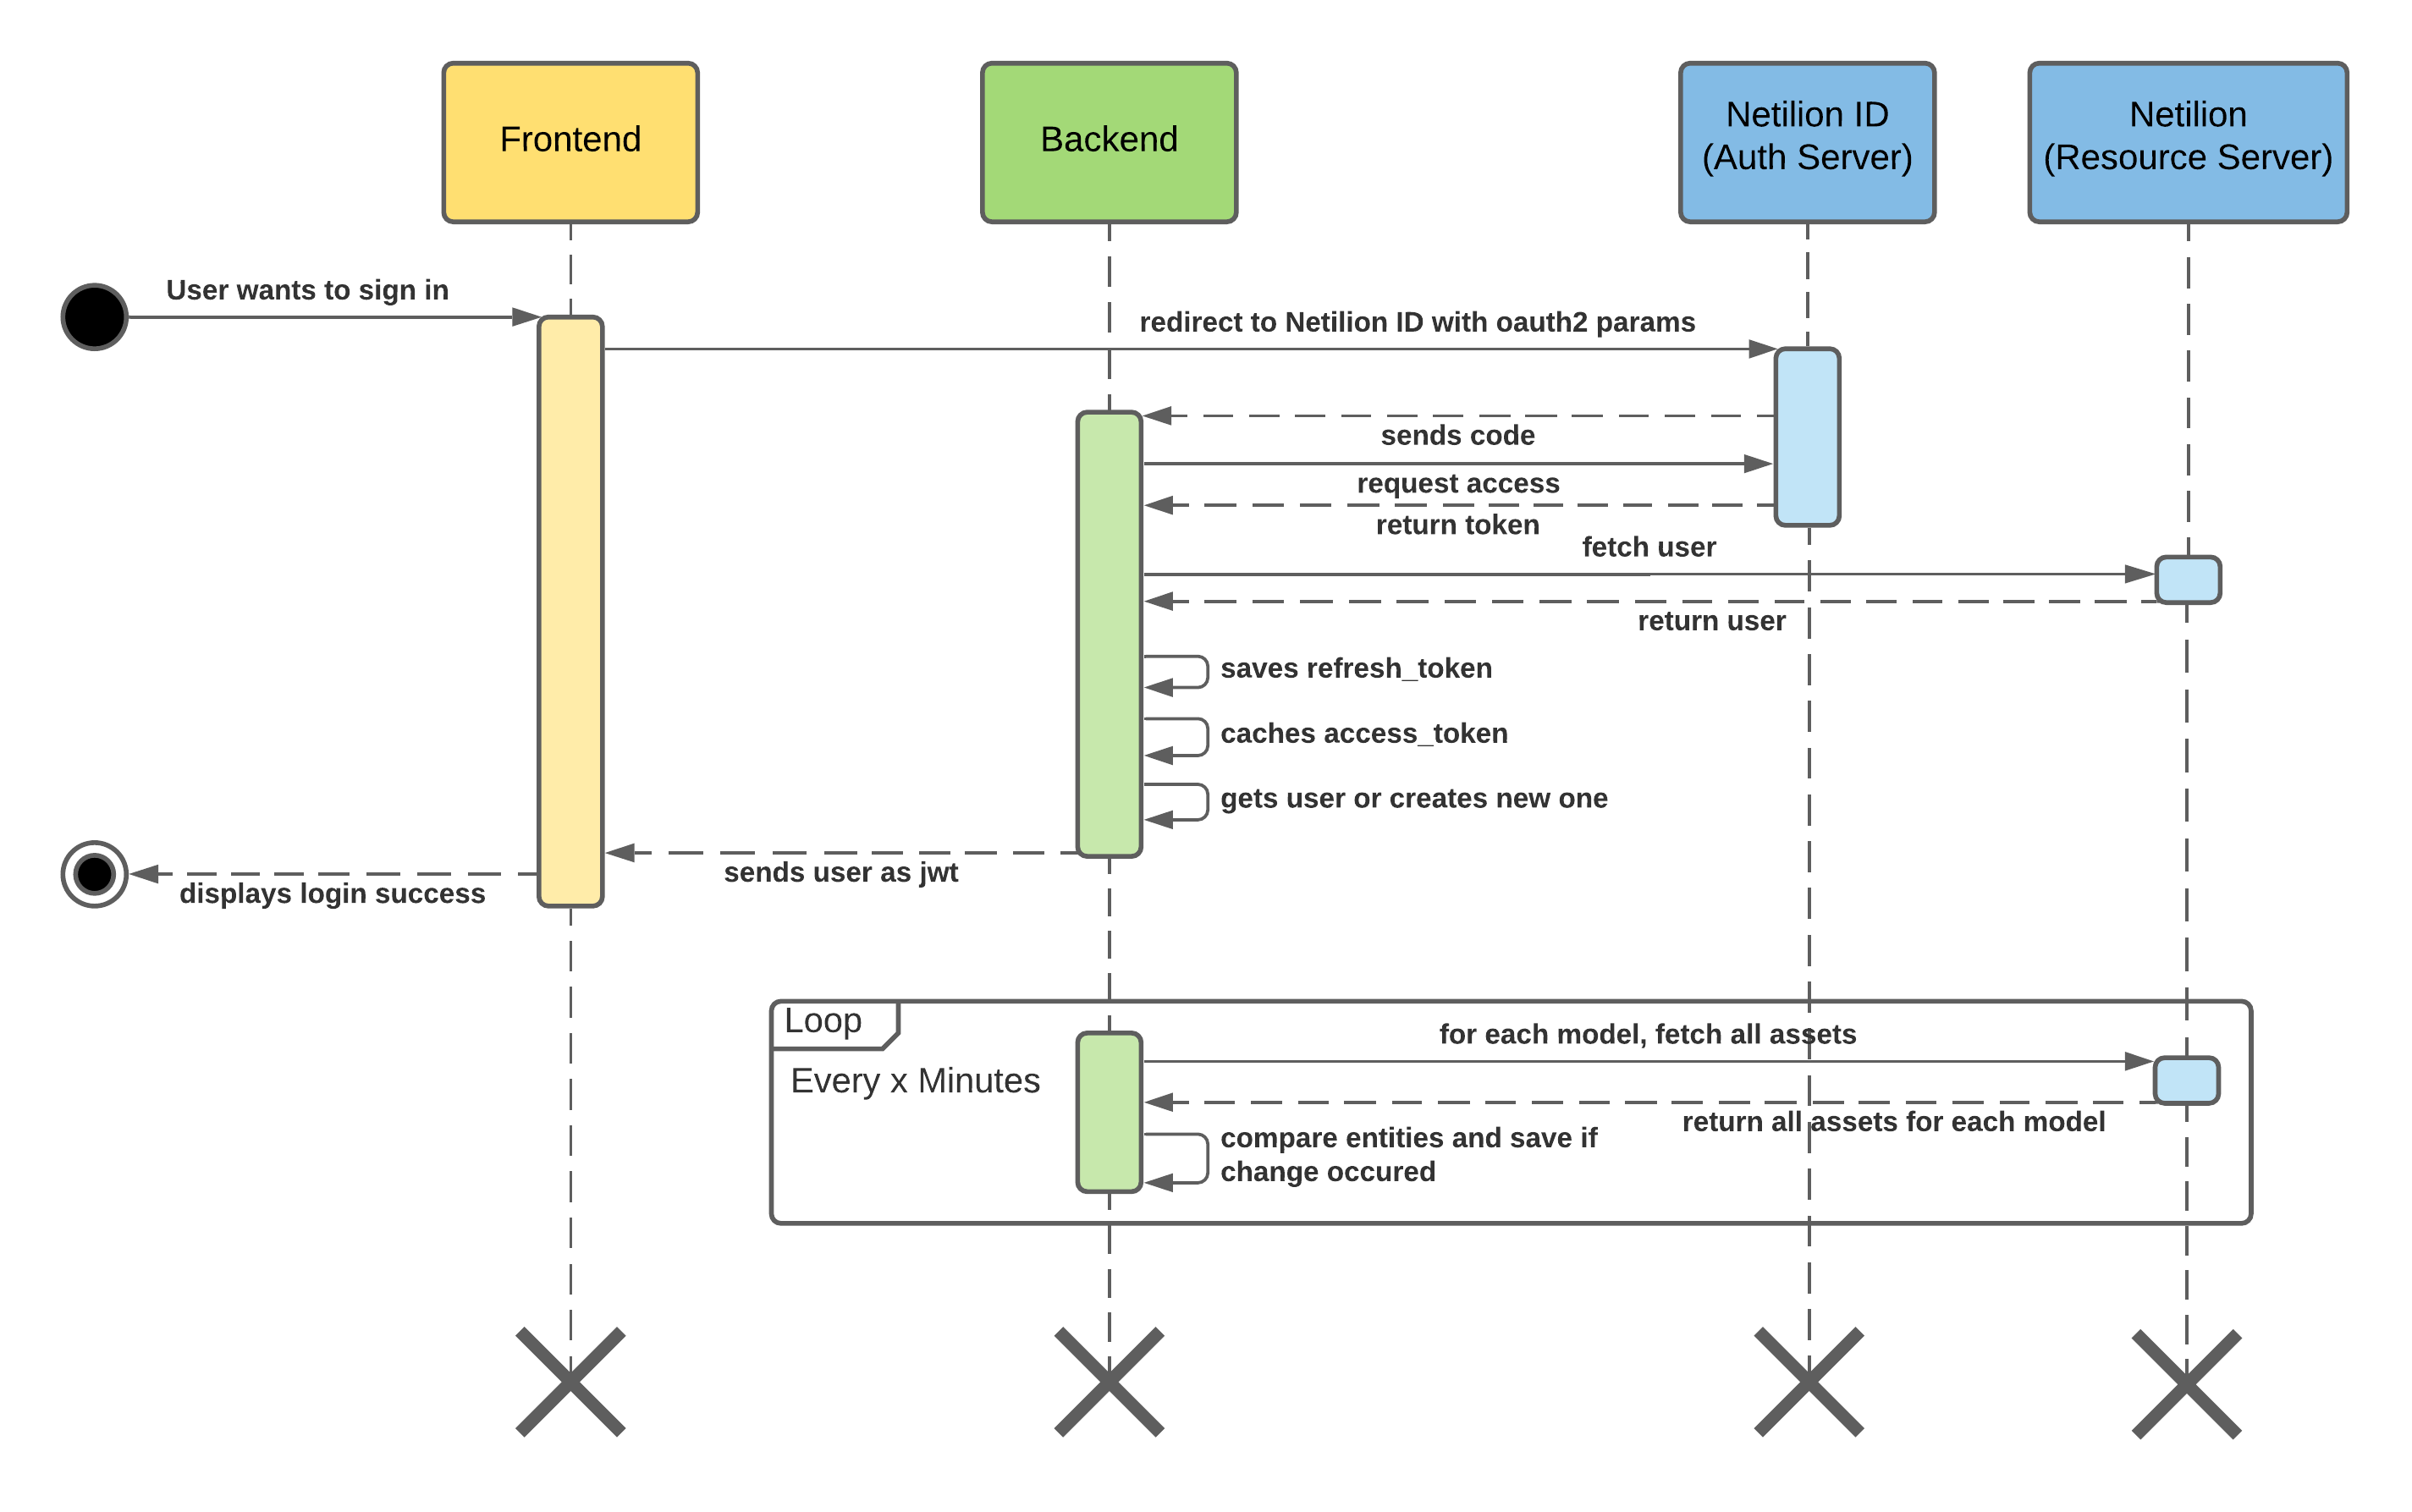
\includegraphics[width=.95\linewidth]{./images/datafetching.png}
  \caption[{Sequenzdiagram, welches das automatische fetching Erklärt}]{Data fetching in Intervallen}
  \label{fig:data-fetching}
\end{figure}
Nachdem sich ein OSE Verantwortlicher das erste mal eingeloggt hat, wird der \code{access\_token} in Redis gecached und der \code{refresh\_token} in der Datenbank gespeichert. Die Funktion soll entweder den gecachten Token nehmen und direkt zurückgeben oder mit dem \code{refresh\_token} einen neuen Anfordern, welcher wiederum gecached und zurückgegeben werden soll. Damit ist es dann möglich, dass das Backend selbst die Daten auffrischen kann. Dafür werde ich das Task-Scheduling\cite{a2021_documentation} feature von Nestjs verwenden. Damit ist es möglich eine Funktion wiederholt laufen zu lassen.
\newline
Bevor ich allerdings das ganze automatisieren kann, brauche ich eine Helferfunktion. Denn jede Anfrage an Netilion braucht einen validen \code{access\_token} und er muss auch dem Netilion Benutzer gehören, unter welchem die Messgeräte registriert sind. Mit dieser Function wird es möglich sein das ganze zu vollautomatisieren. Wenn nun ein Benutzer des OSE-Dashboards sich die Daten nun ansehen möchte, kann er dies machen, ohne den Login des jeweiligen OSE Verantwortlichen wissen zu müssen.
\pagebreak
\subsection{Zugriffskontrolle}
\subsubsection{OSE Verantwortlicher}
\begin{figure}[H]
  \centering
  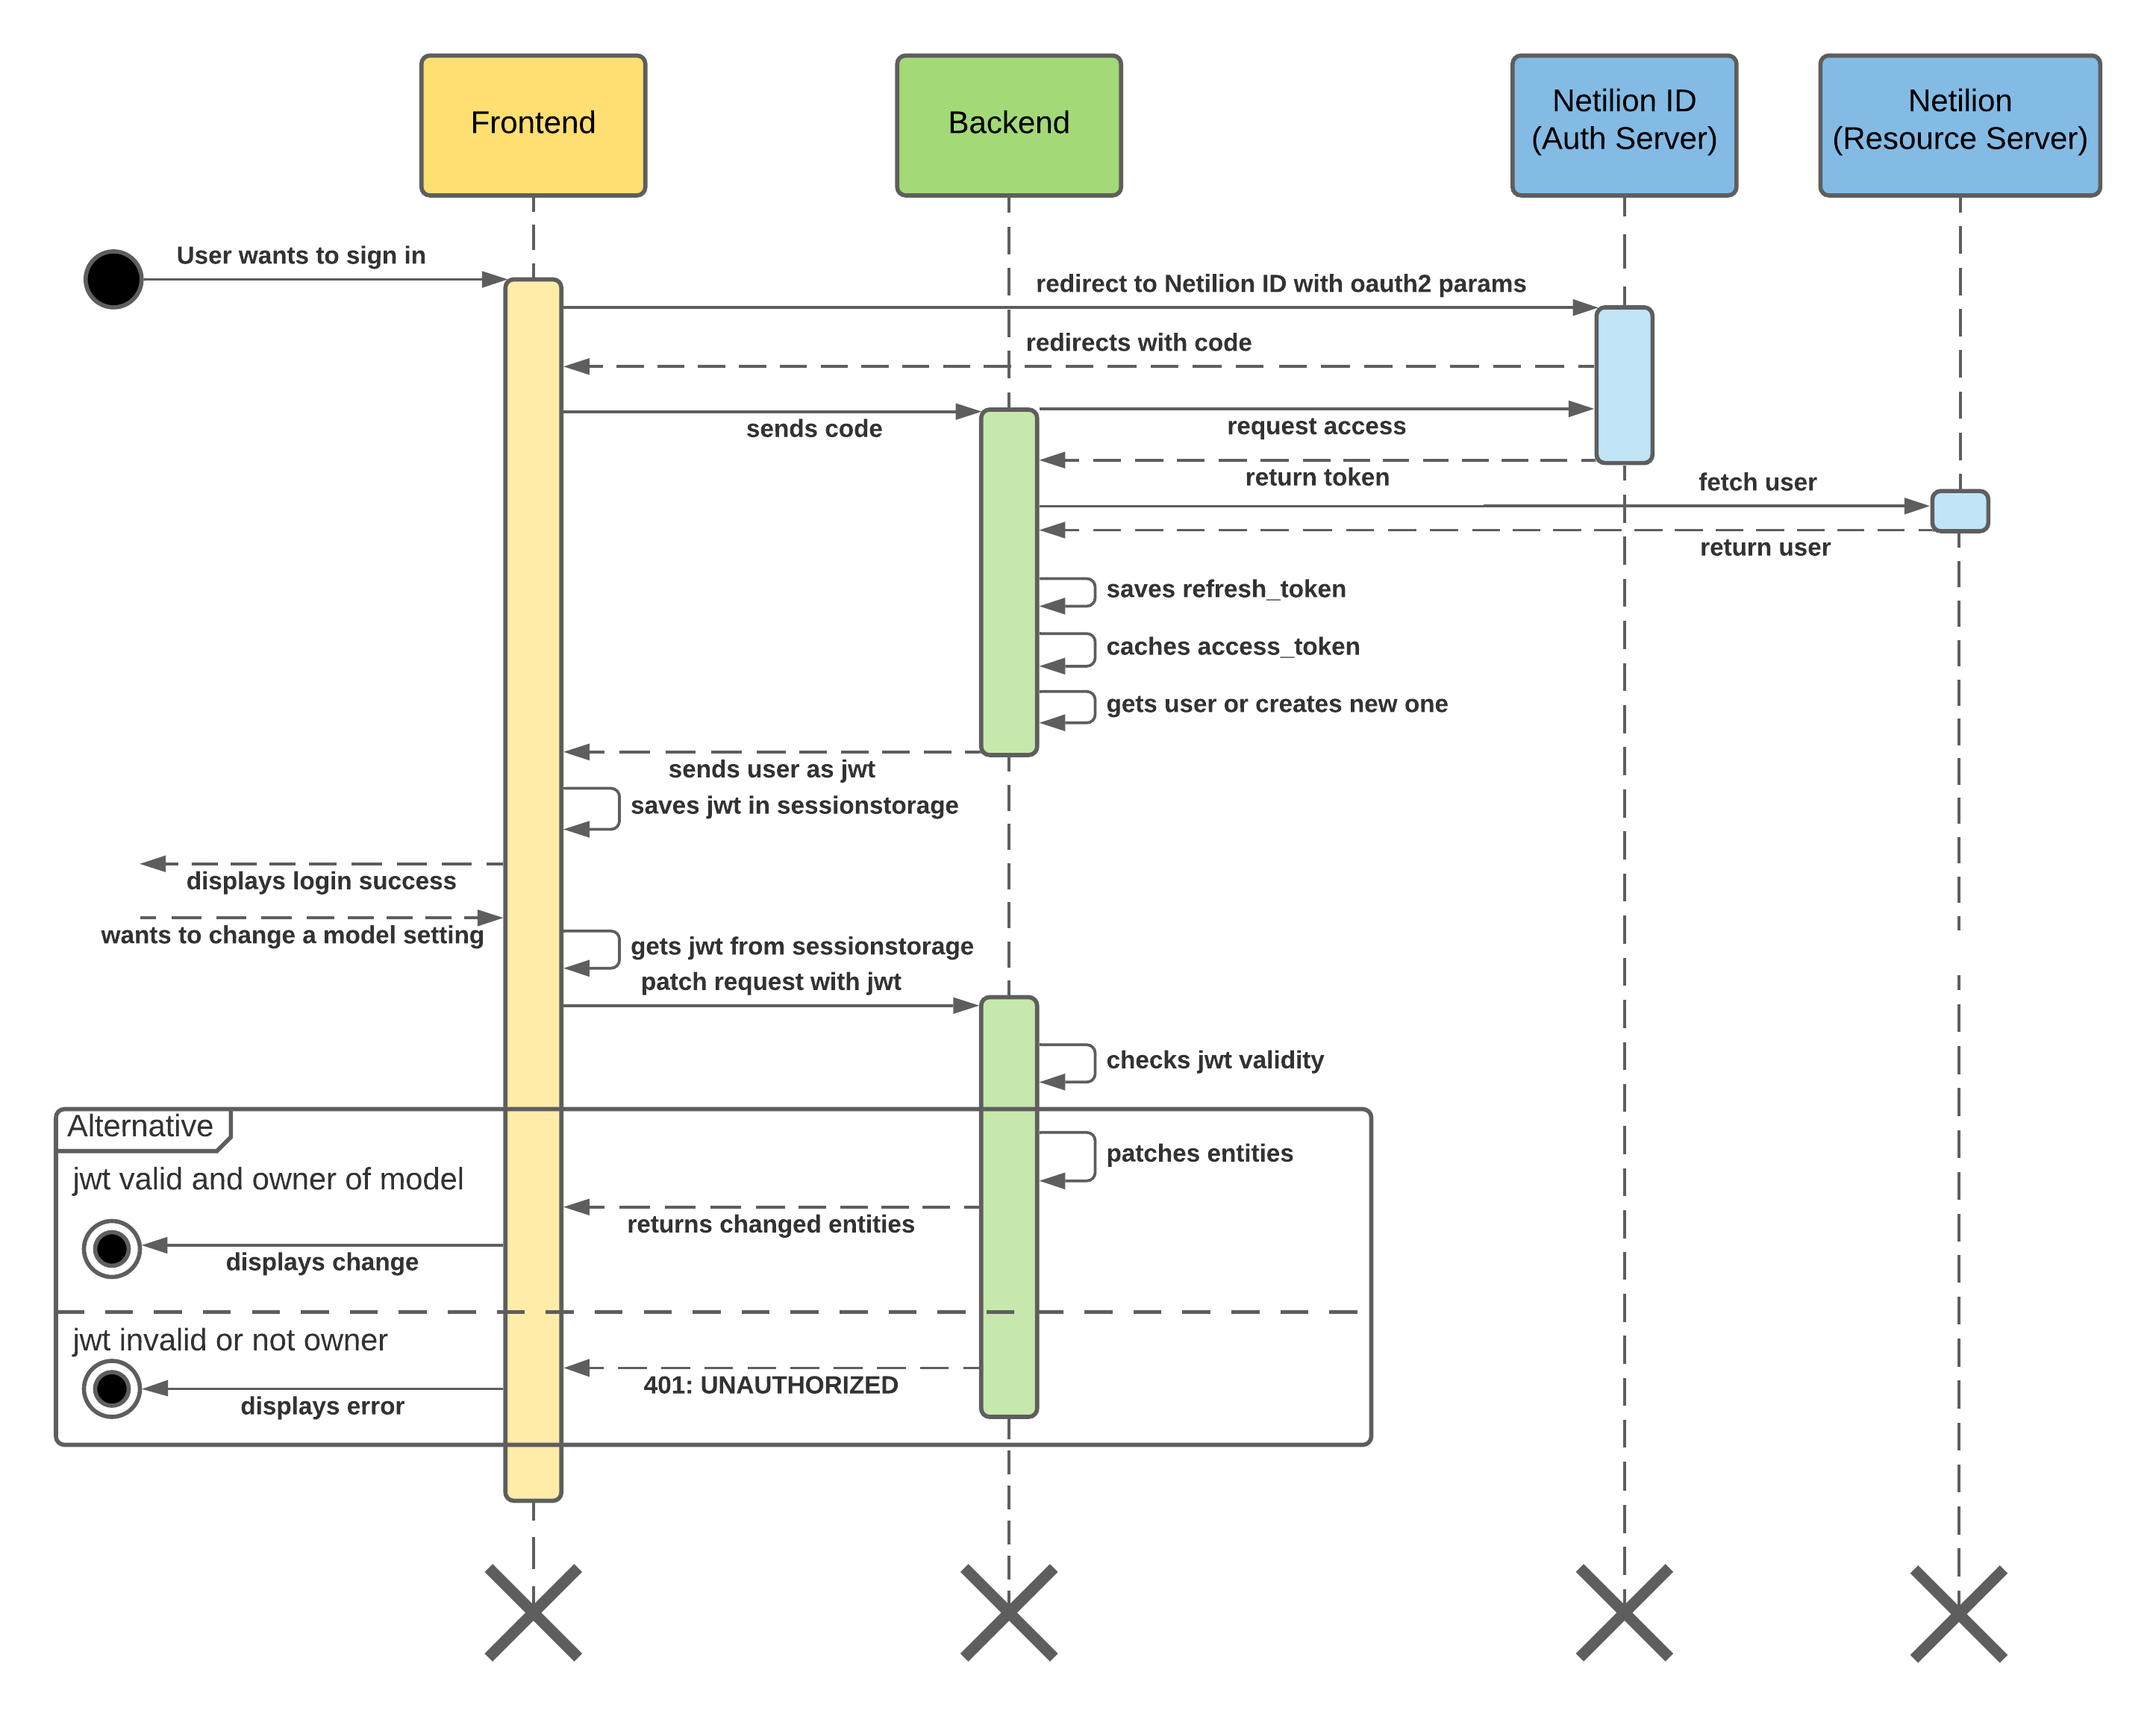
\includegraphics[width=.95\linewidth]{./images/zugriffskontrolle.png}
  \caption[{Sequenzdiagram, welches die Zugriffskontrolle für den OSE Verantwortlichen beschreibt}]{Zugriffskontrolle OSE Verantwortlicher}
  \label{fig:zugriffskontrolle}
\end{figure}
Ein OSE Verantwortlicher soll das Konfigurationsmenü seines Models öffnen können. Verantwortlicher anderer Modelle oder normale User sollen dies nicht können.
Das ganze sollte folgenderweise gelöst werden:
\newline
Das Frontend erhält nach dem erfolgreichen Login einen JWT. Dieser wird zuerst benötigt, um den Link zum Konfigurationsmenü überhaupt erst im Frontend anzuzeigen. Ausserdem wird er als Authentifizierungsmethode zum Backend verwendet. Der REST Endpoint vom Backend wird durch eine Nestjs Guard\cite{nest_guards} geschützt. Daraufhin wird direkt geprüft werden, ob das Model auch wirklich dem User gehört. Sollte dies nicht der Fall sein, wird die Anfrage als unauthorized zurückgeschickt.
\subsubsection{OSE-Dashboard Nutzer}
\begin{figure}[H]
  \centering
  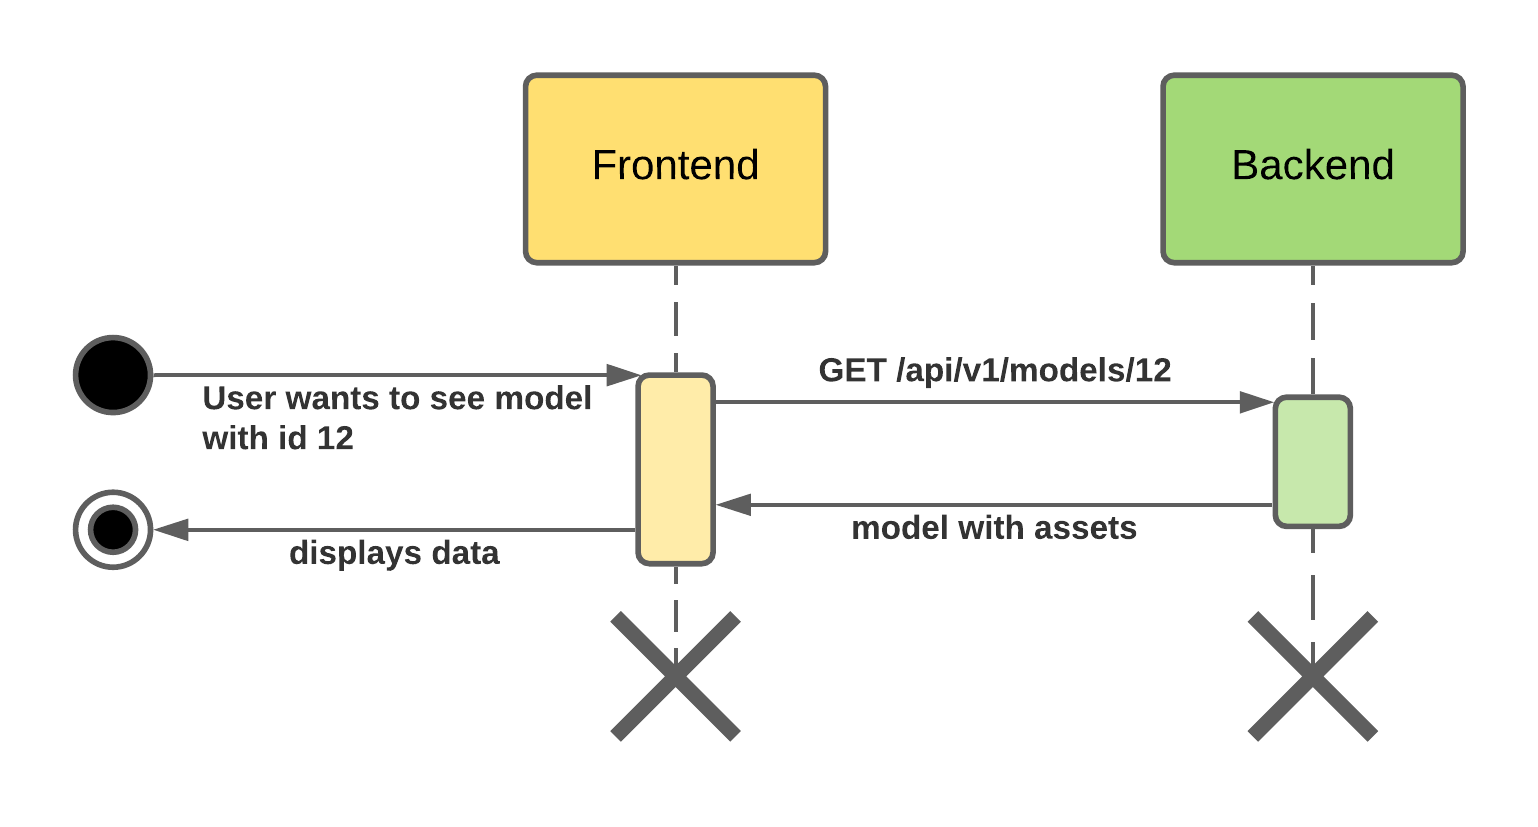
\includegraphics[width=.6\linewidth]{./images/zugriffskontrolle2.png}
  \caption[{Sequenzdiagram, welches die Zugriffskontrolle für den OSE-Dashboard Nutzer beschreibt}]{Zugriffskontrolle OSE-Dashboard Nutzer}
  \label{fig:zugriffskontrolle2}
\end{figure}
Der OSE-Dashboard möchte sich alle OSE-Modelle ansehen können, ohne sich dabei einloggen zu müssen.
Das ganze sollte folgenderweise gelöst werden:
\newline
Wie in Kapitel \ref{data-fetching} angesprochen, sind die aktuellen Daten im Backend verfügbar. So ist es also gar nicht nötig Netilion direkt anzufragen. Das Backend soll stattdessen die Daten mit einem public Endpoint verfügbar machen. Auf diesem Weg umgehen wir auch die maximale Anfragen an Netilion, welche in Kapitel \ref{arch-backend} beschrieben wurde.
\newline
So kann das Frontend beliebig oft die Daten abfragen, ohne das sich ein User einloggen muss oder das wir die Grenze der Connect Subscription übertreten.
\section{Mockups}
Mockups dienen zur Planung der Darstellung des Frontends. Es ist viel sinnvoller das Layout und den Inhalt der Website im Vorfeld zu skizzieren und damit herumzuspielen, als während dem Implementieren. Weiss man während der Implementierungsphase noch nicht wie das Produkt grob aussehen sollte verschwendet man meist wertvolle Zeit.
\newline
Oft wird vor der Erstellung der Website ein UX-Design erstellt. Dieses gibt grob das Layout und den Inhalt. Ein UI-Design wird angewand wenn das detaillierte Design der Website wichtig ist. Dabei werden die ganzen Komponenten der Website bis ins Detail im Vorfeld designed, sodass dies den Anspruchsgruppen und den Programmieren klar ist.
\newline
Bei dieser Arbeit ist nur die Erarbeitung eines UX-Designs wichtig. Dies wurde soweit erstellt und ist nachfolgend in den Kapiteln dokumentiert.
\pagebreak
\subsection{Index Page} \label{mck:index} 
Momentan ist die Index Page des OSE-Dashboards das Reinacher Model selbst. Dies soll sich nun ändern. Die rote Linie markiert die initiale Sicht des User. Diese enthält den Titel und eine Beschreibung der Webapplikationen, gefolgt von der Auswahlmöglichkeit der ganzen Modelle. Unter der initialen Sicht ist ein Abschnitt, welcher den User fragt, ob er für ein OSE-Model zuständig ist. Sollte dies der Fall sein, könne er sich einloggen und so die Daten für das Dashboard zur verfügung stellen.
\begin{figure}[H]
  \centering
  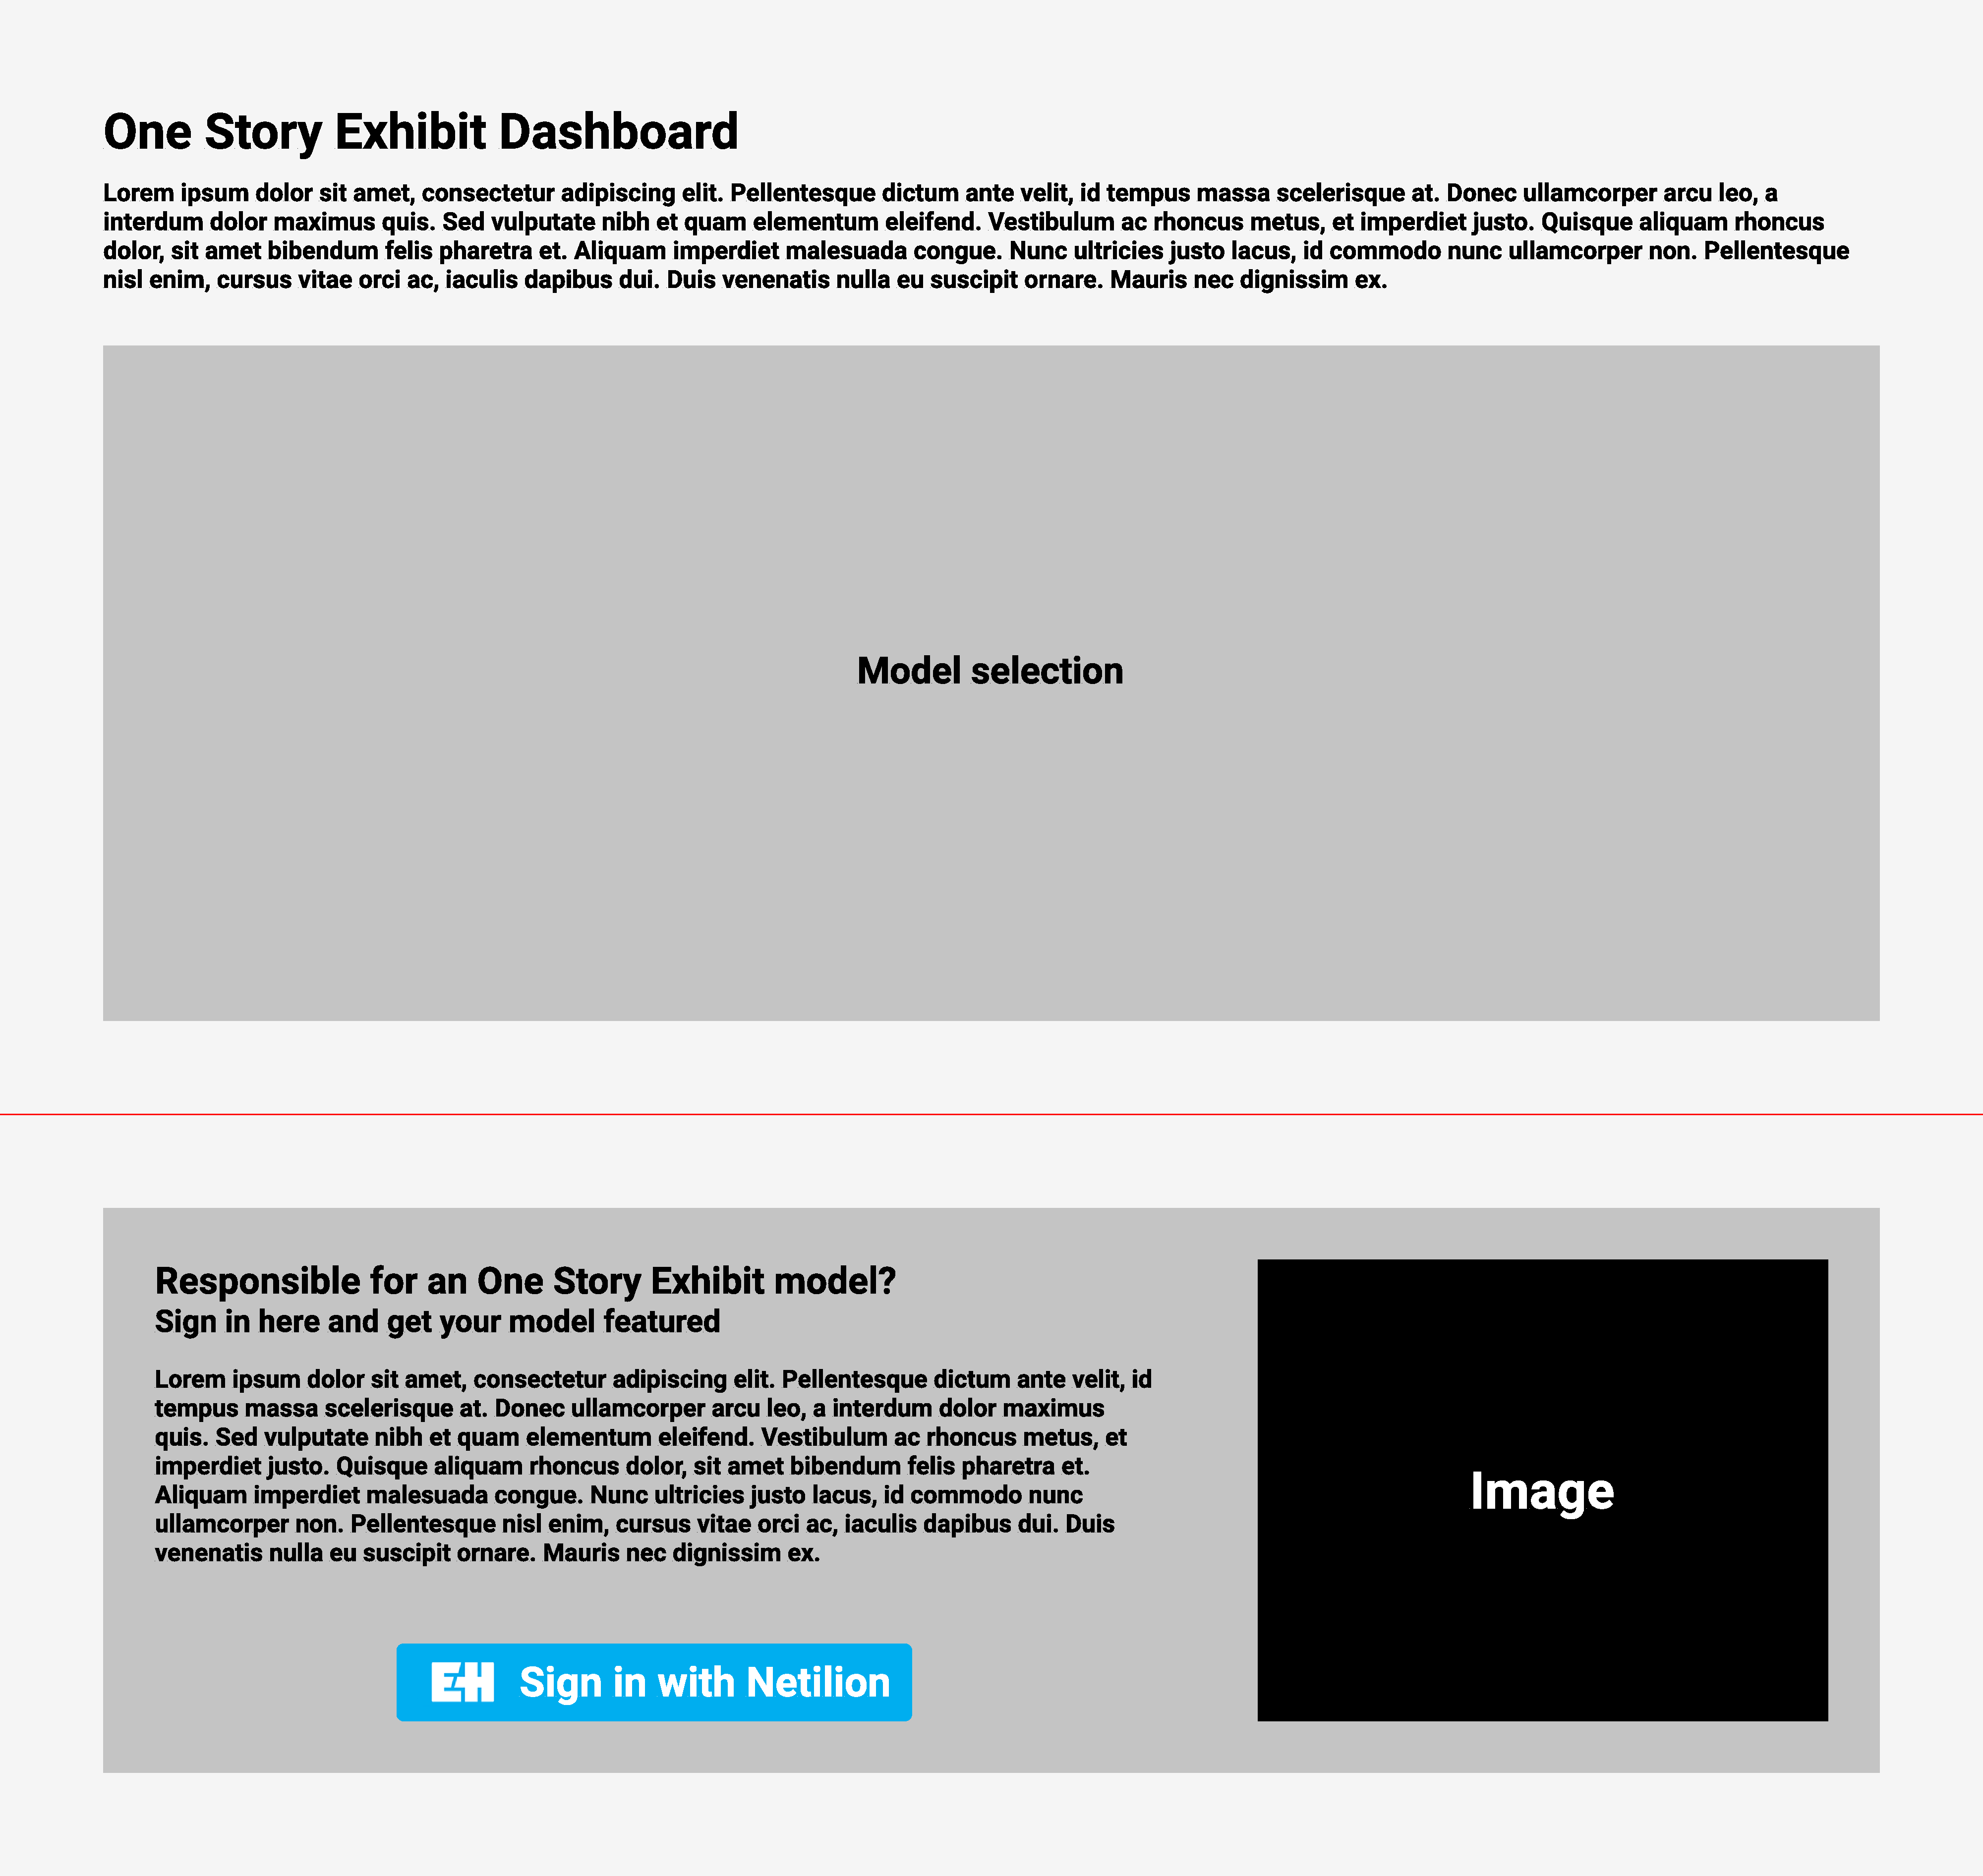
\includegraphics[width=\textwidth]{./mockups/index/not_signed_in.pdf}
  \caption[{Mockup der Index Page}]{Mockup der Index Page}
  \label{fig:mck-index}
\end{figure}
\pagebreak
\subsection{Registration} \label{mck:registration}
\subsubsection{Fehlermeldung}
Sollte beim Loginprozess etwas schiefgehen, wird die unten dargestellte Fehlermeldung angezeigt. Dabei wird erwähnt, dass dieser Fehler sehr wahrscheinlich durch den Kandidaten geschah und nicht durch Netilion. Darunter befindet sich die Meldung, dass der User in x Sekunden wieder auf die Startseite weitergeleited wird.
\begin{figure}[H]
  \centering
  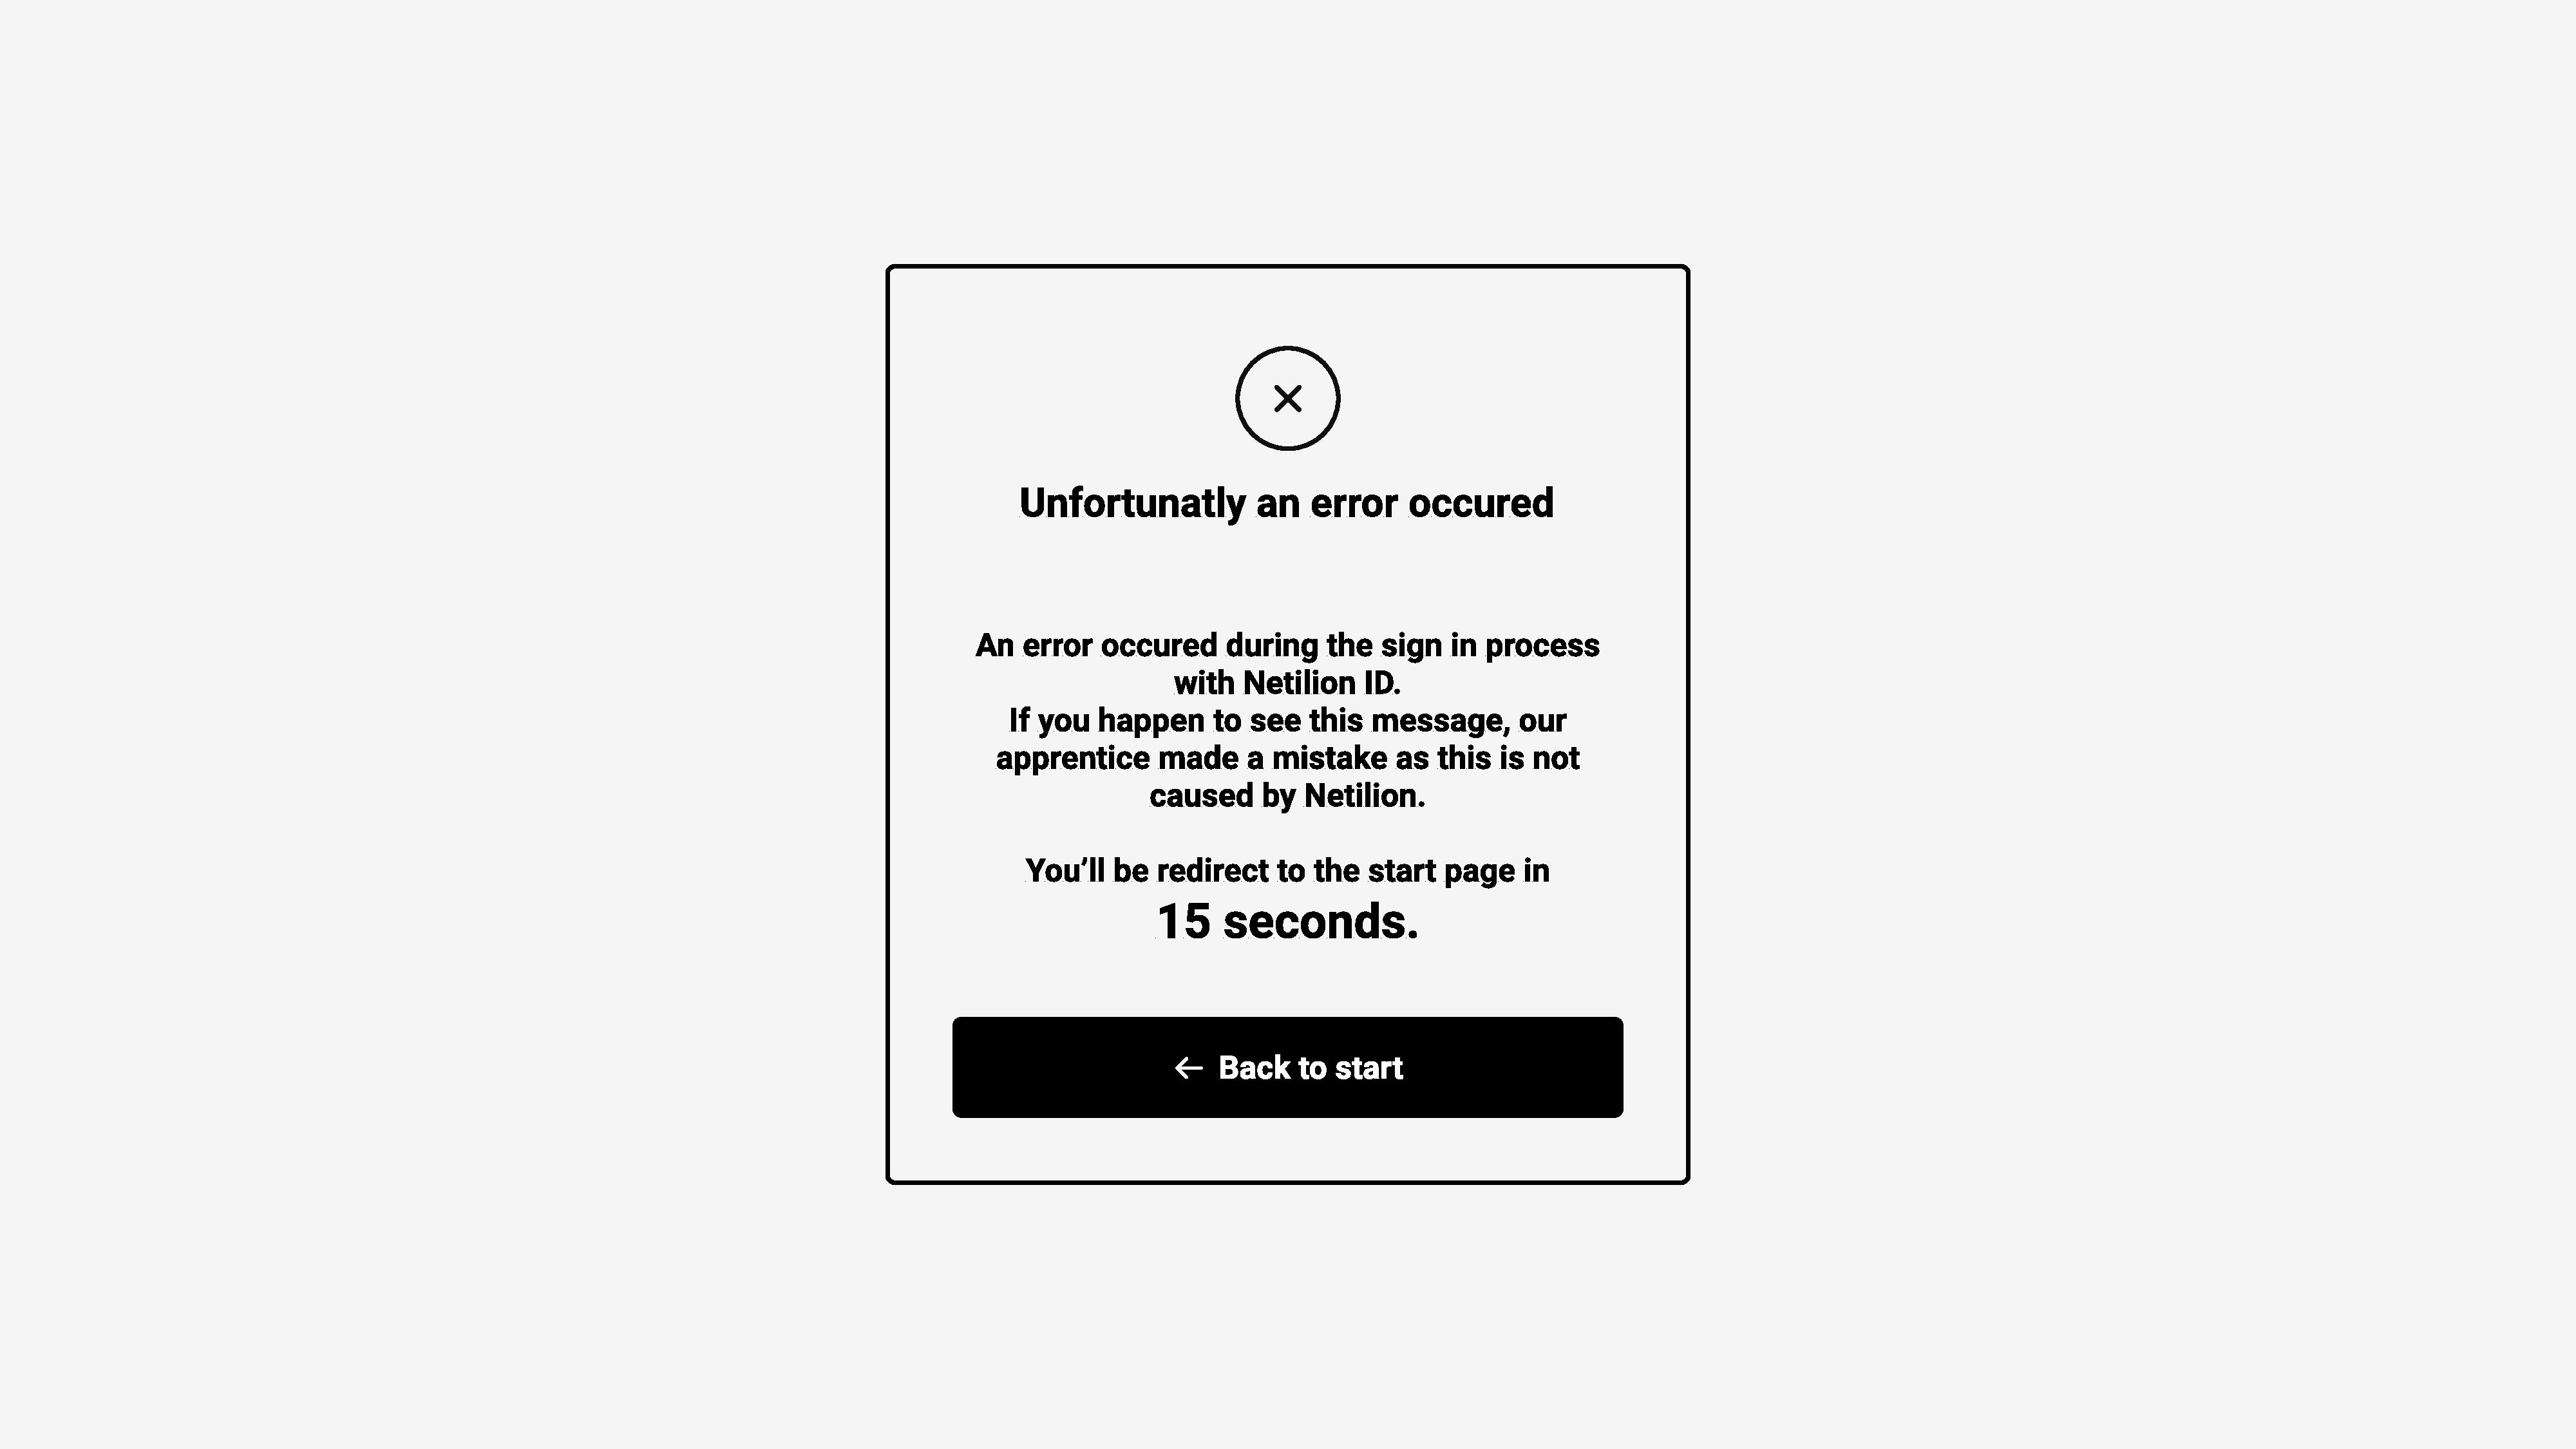
\includegraphics[angle=270,width=0.6\textwidth]{./mockups/register/error.pdf}
  \caption[{Mockup einer Fehlermeldung}]{Mockup einer Fehlermeldung}
  \label{fig:mck-error}
\end{figure}
\pagebreak
\subsubsection{Anmeldung erfolgreich}
Diese Ansicht wird angezeigt, wenn der Loginprozess erfolgreich abläuft. Dabei wird im oberen Teil angezeigt, dass dies der Erste der insgesammt drei Schritte ist, welche für die erfolgreiche Registration benötigt werden.
\begin{figure}[H]
  \centering
  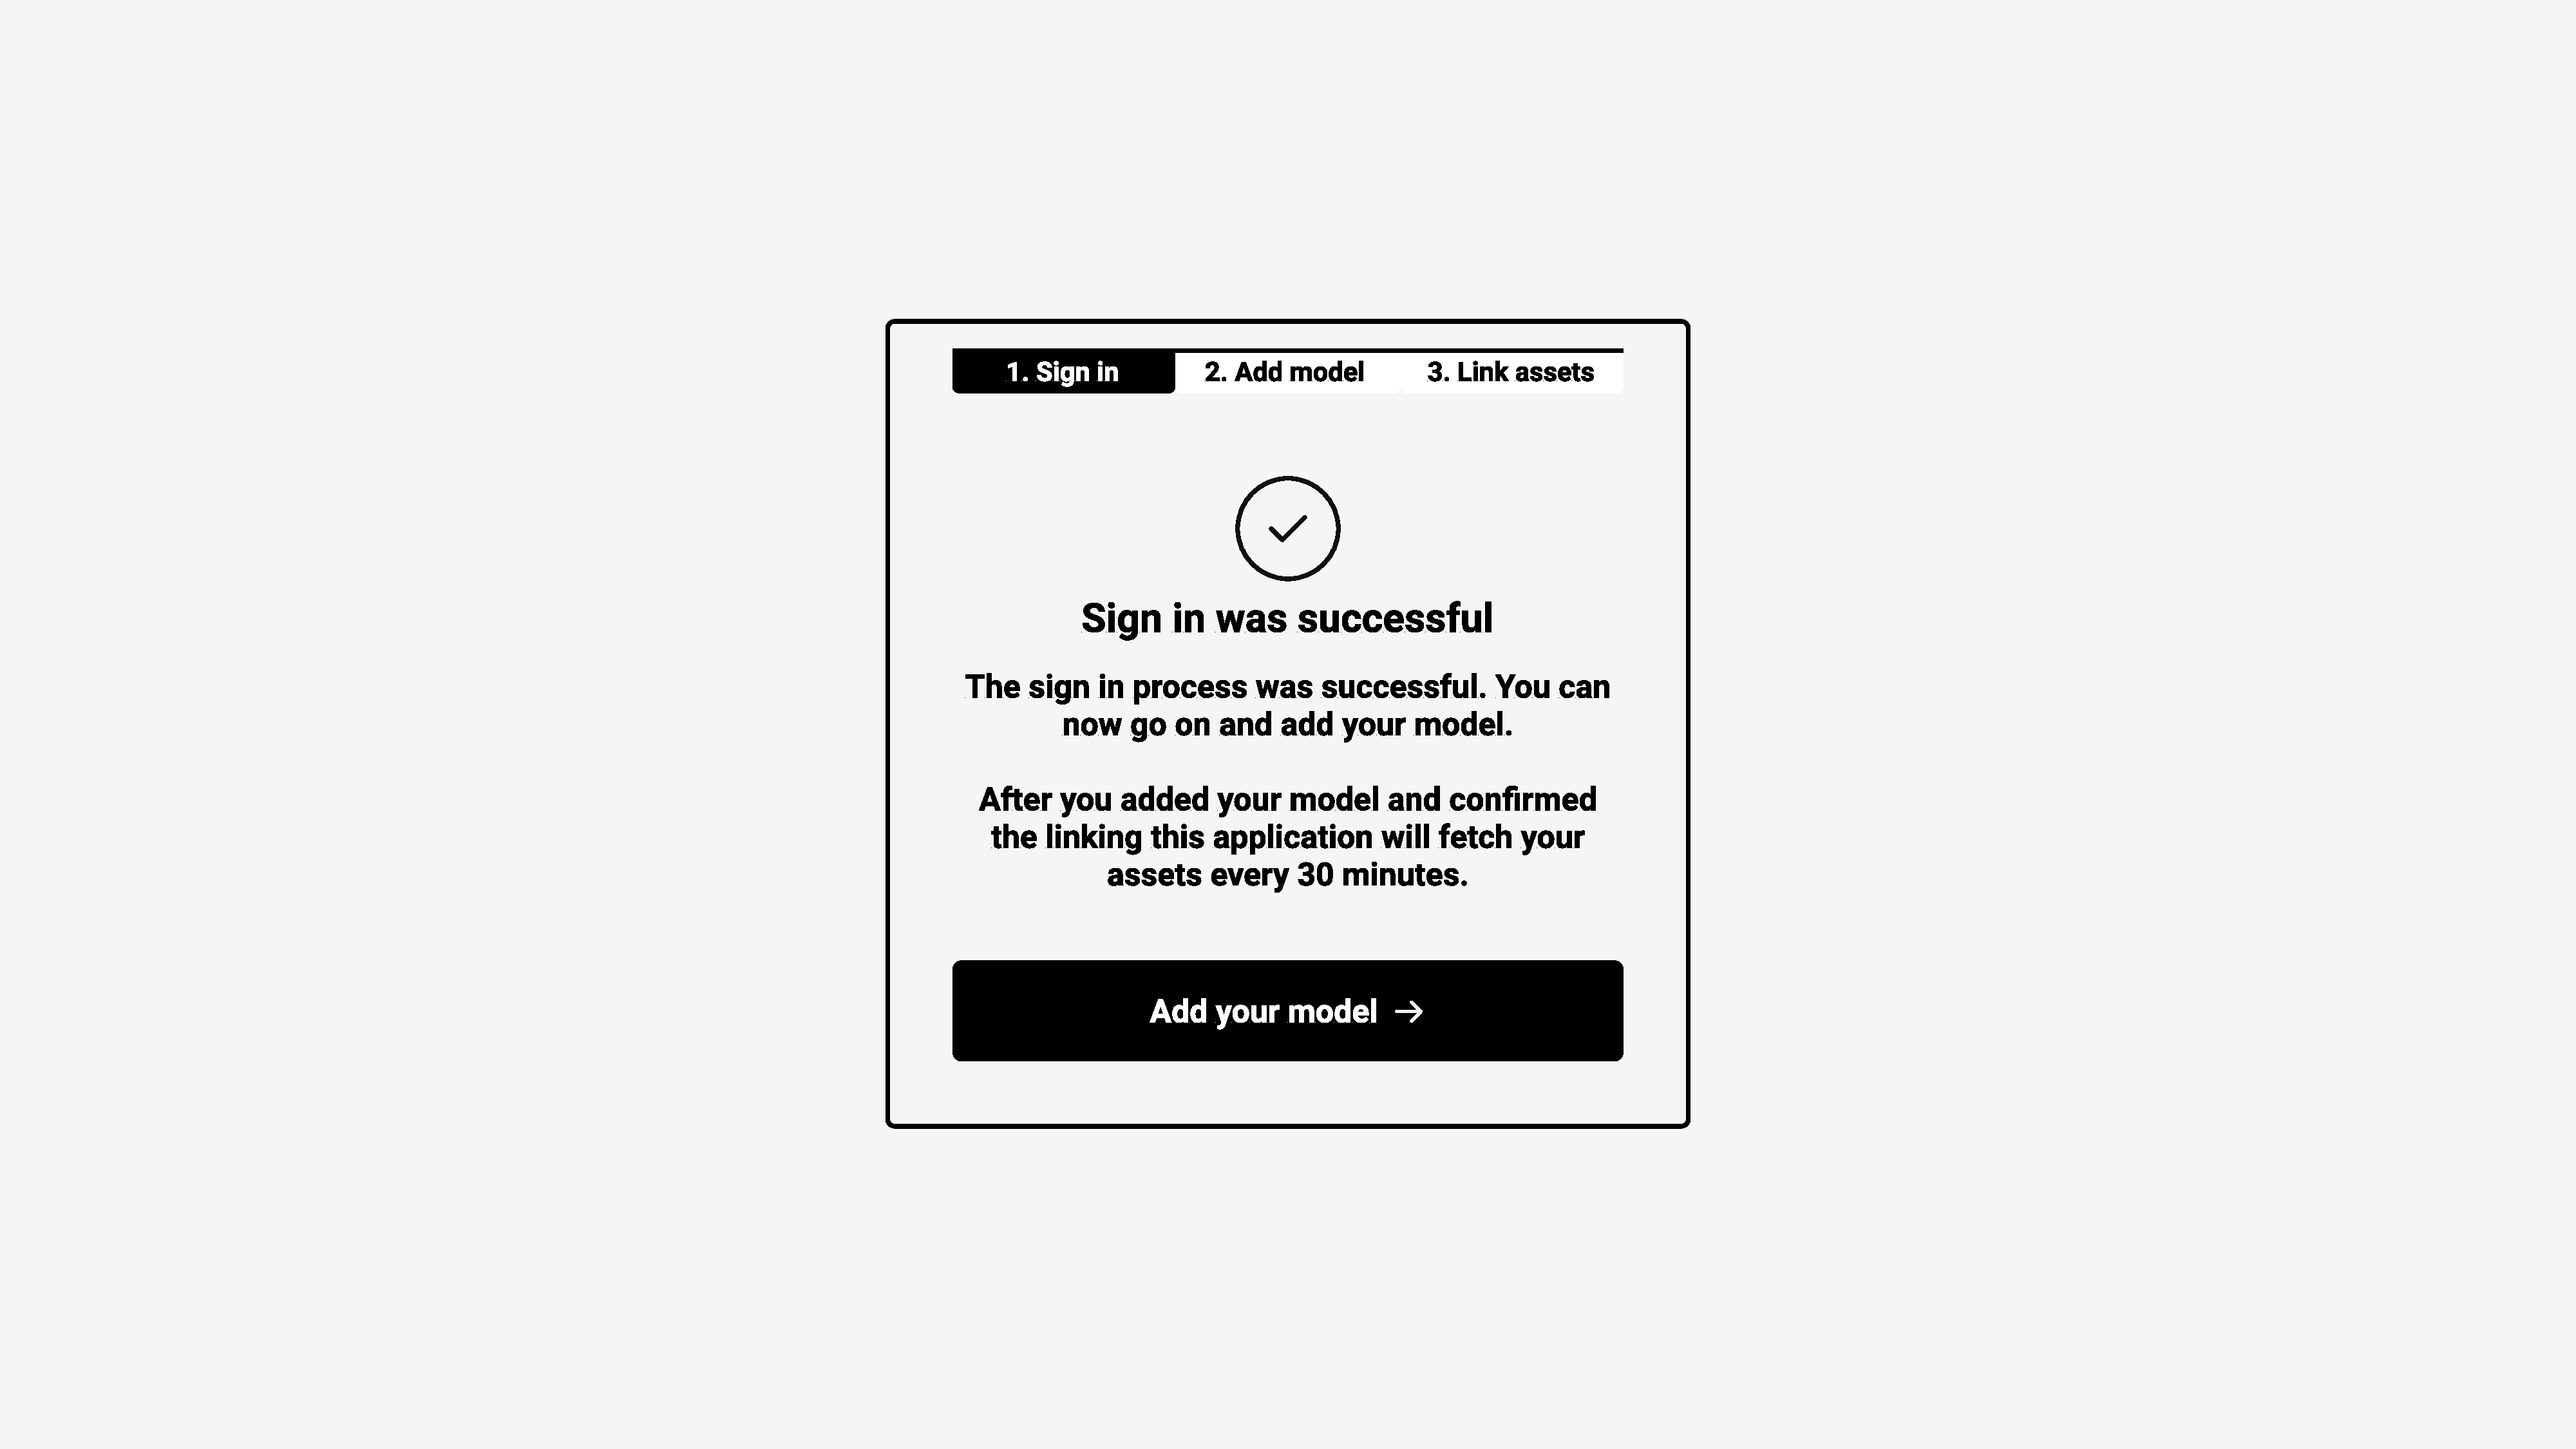
\includegraphics[angle=270,width=0.6\textwidth]{./mockups/register/stage_1.pdf}
  \caption[{Mockup einer erfolgreichen Anmeldung}]{Mockup einer erfolgreichen Anmeldung}
  \label{fig:mck-stage_1}
\end{figure}
\pagebreak
\subsubsection{Model registrieren}
Nun wird der OSE-Verantwortlicher darum gebeten, seinem Model einen Namen zu geben und den Standort anzugeben, damit die User sein Model dann über die Index Page finden können.
\begin{figure}[H]
  \centering
  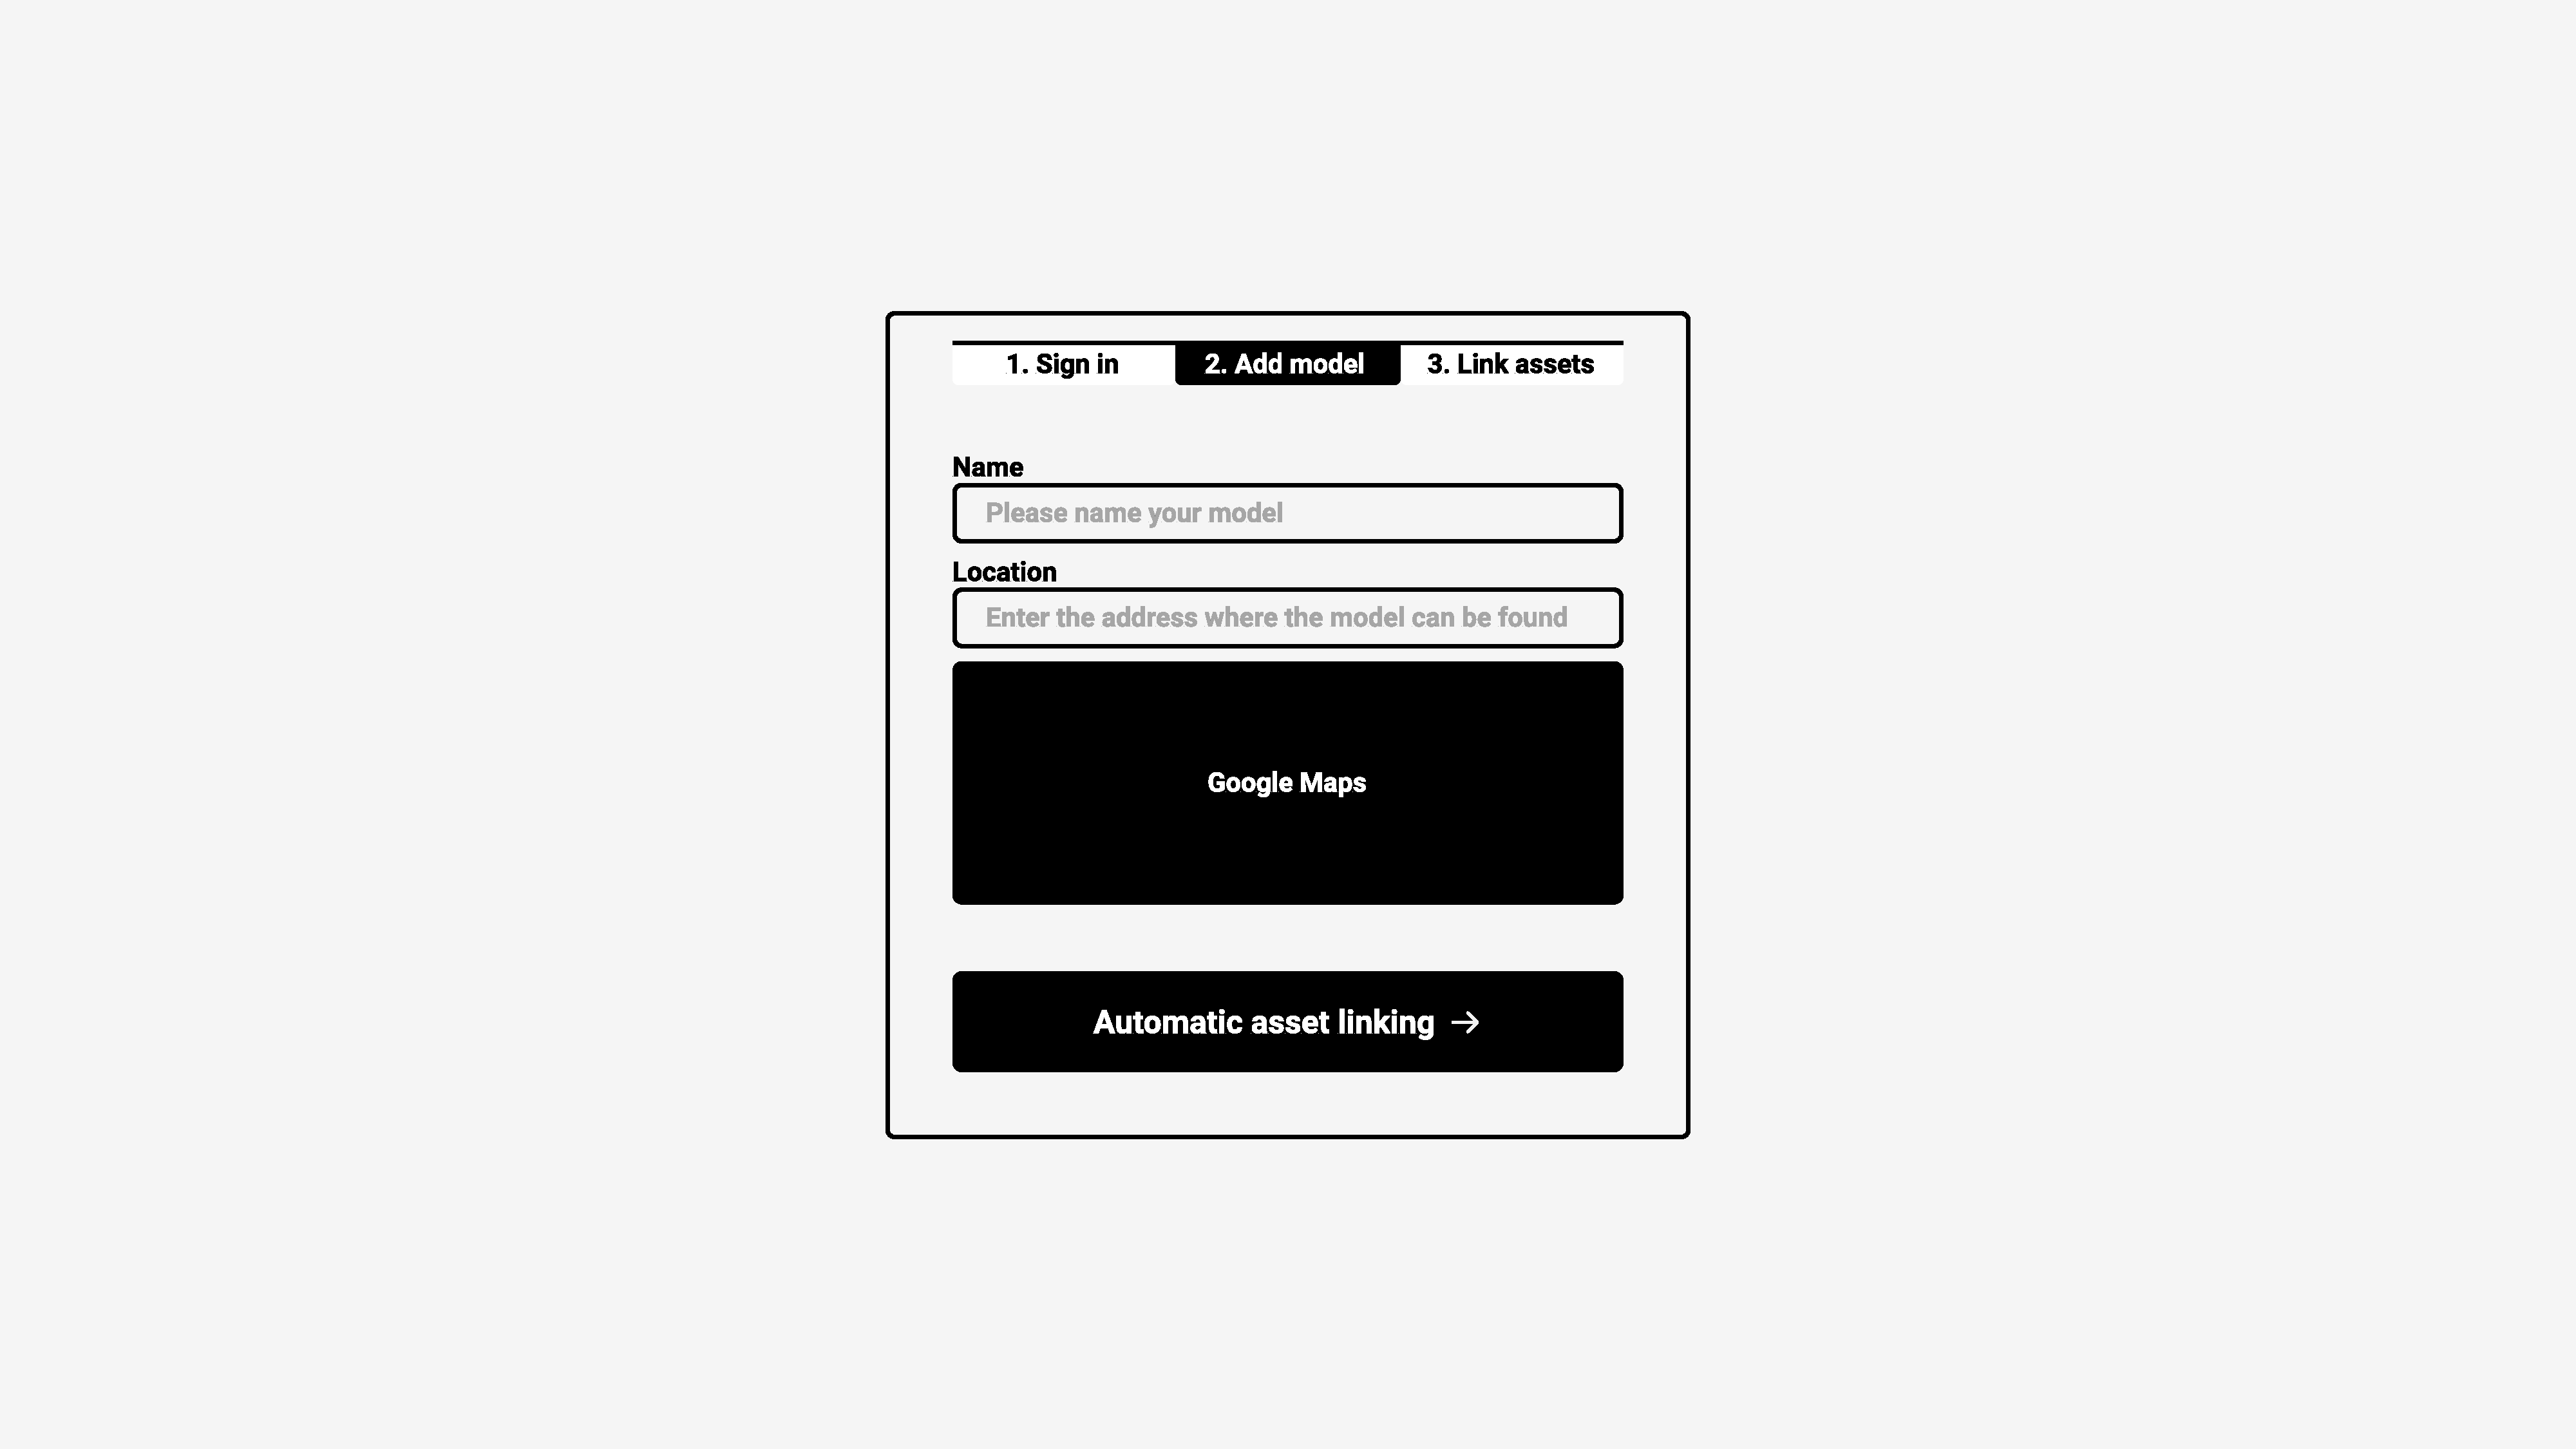
\includegraphics[angle=270,width=0.6\textwidth]{./mockups/register/stage_2.pdf}
  \caption[{Mockup der Registration}]{Mockup der Registration}
  \label{fig:mck-stage_2}
\end{figure}
\pagebreak
\subsubsection{Asset verlinkung}
Der letzte Schritt der Registrierung ist das Verlinken der Assets mit den Meshes des 3D Models. Da dies automatisch geschieht, wird der User an dieser stelle gebeten zu warten, bis der Prozess abgeschlossen ist.
\begin{figure}[H]
  \centering
  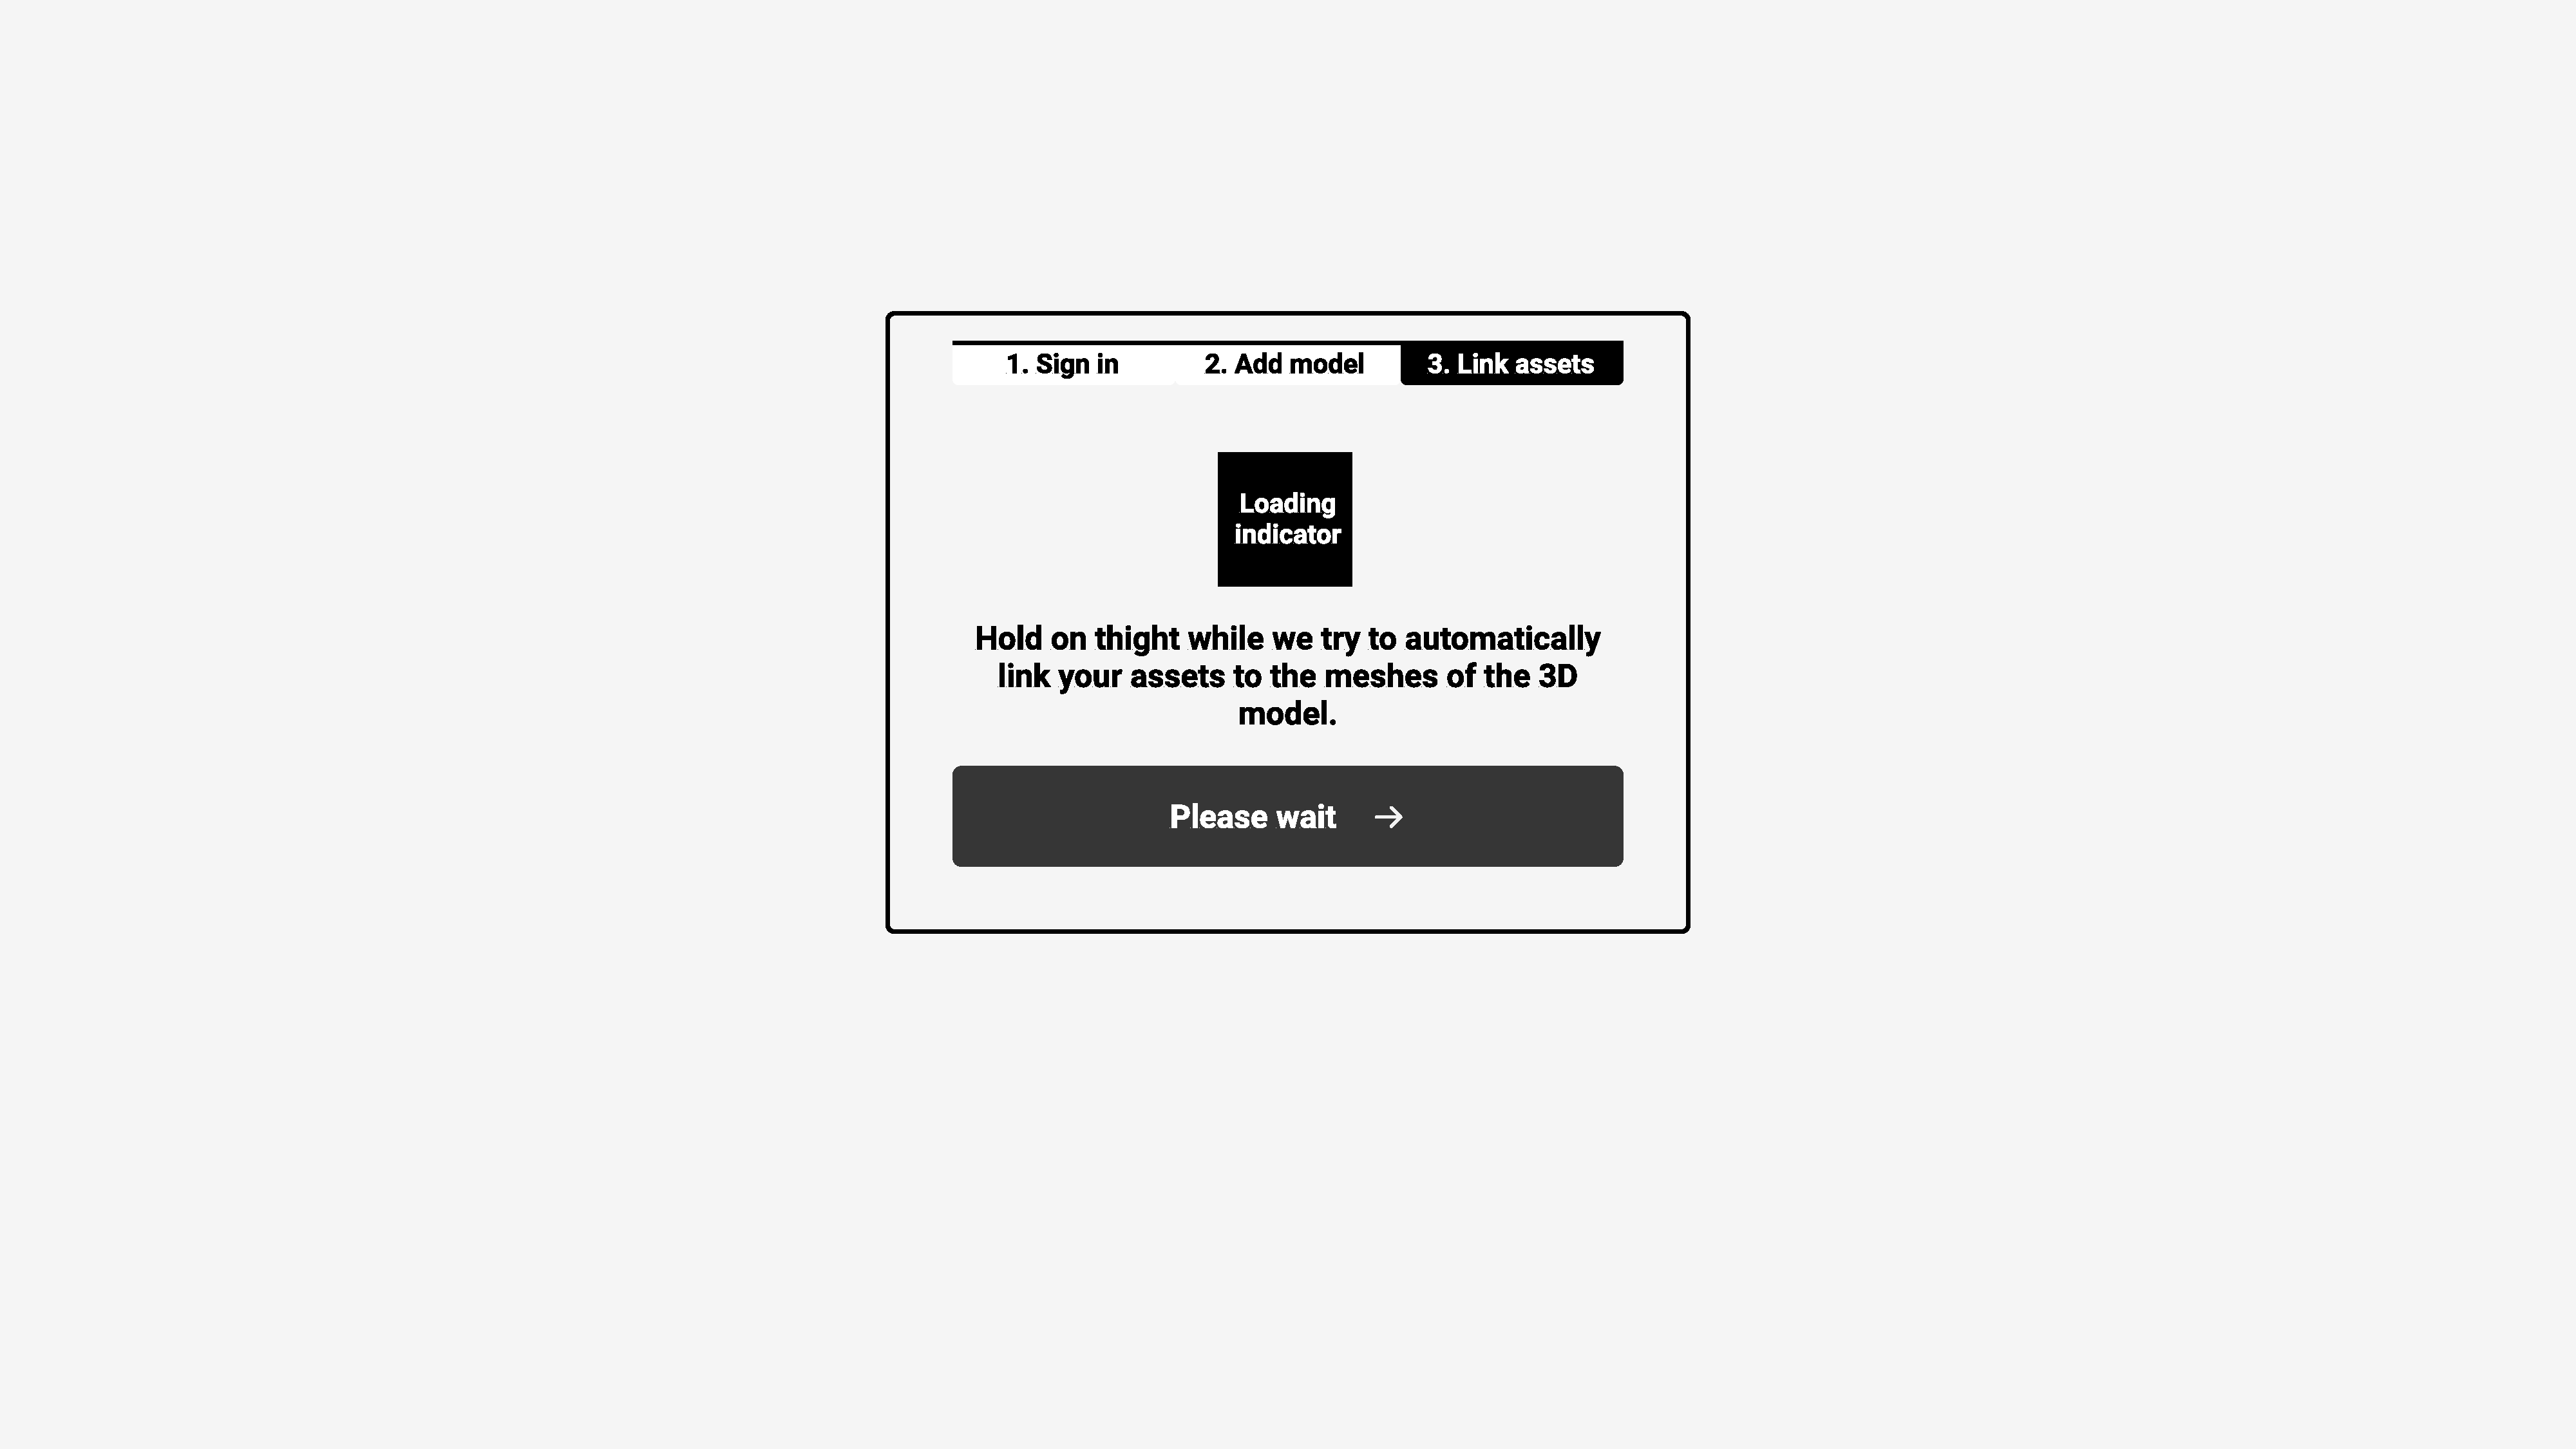
\includegraphics[angle=270,width=0.6\textwidth]{./mockups/register/stage_3.pdf}
  \caption[{Mockup der Asset verlinkung}]{Mockup der Asset verlinkung}
  \label{fig:mck-stage_3}
\end{figure}
\pagebreak
\subsubsection{Asset verlinkung fehlgeschlagen}
Konnten nicht alle Assets verlinkt werden, wird dieses Fenster angezeigt. Es erklärt dem User was geschah und das er die Verlinkung im nächsten Schritt manuel anpassen kann.
\begin{figure}[H]
  \centering
  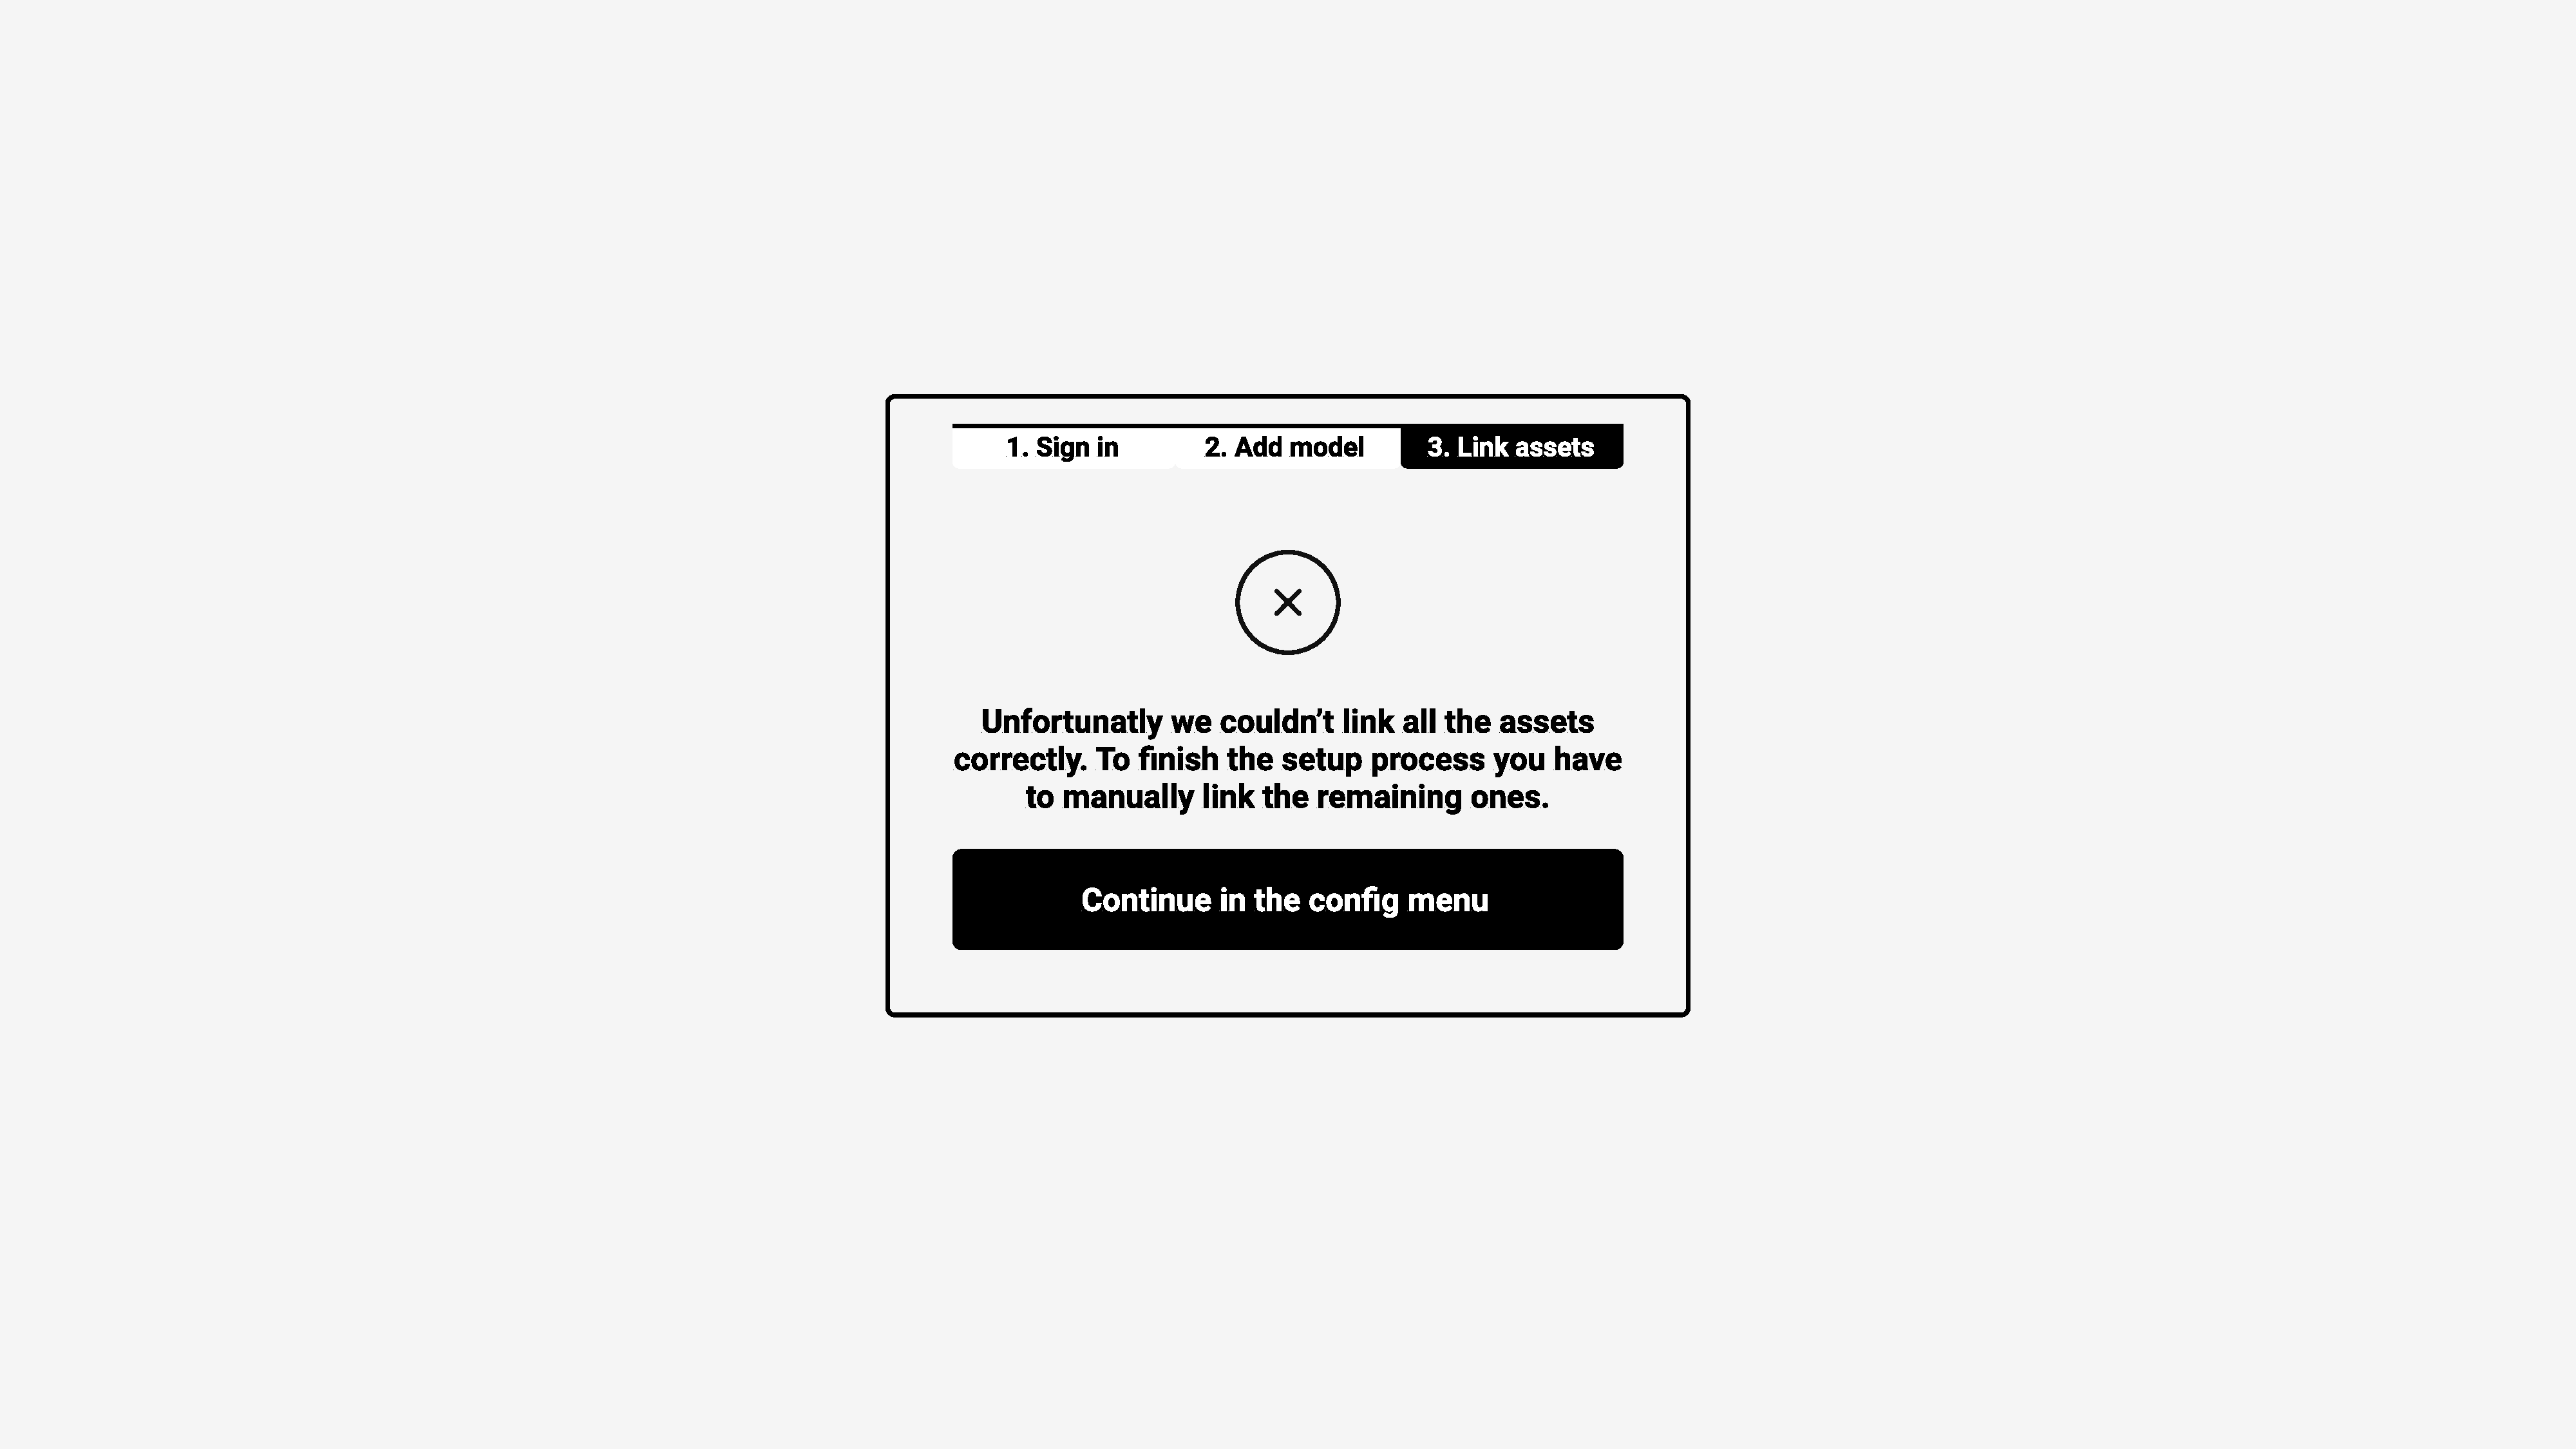
\includegraphics[angle=270,width=0.6\textwidth]{./mockups/register/redirect.pdf}
  \caption[{Mockup einer fehlgeschlagenen Verlinkung}]{Mockup einer fehlgeschlagenen Verlinkung}
  \label{fig:mck-redirect}
\end{figure}
\pagebreak
\subsubsection{Asset verlinkung erfolgreich}
Konnten alle Assets verlinkt werden, wird dieses Fenster angezeigt. Es informiert den User, dass der Registrationsprozess hiermit abgeschlossen ist. Mit dem Knopf am unteren Rand wird er ausgeloggt und kehrt zur Startseite zurück.
\begin{figure}[H]
  \centering
  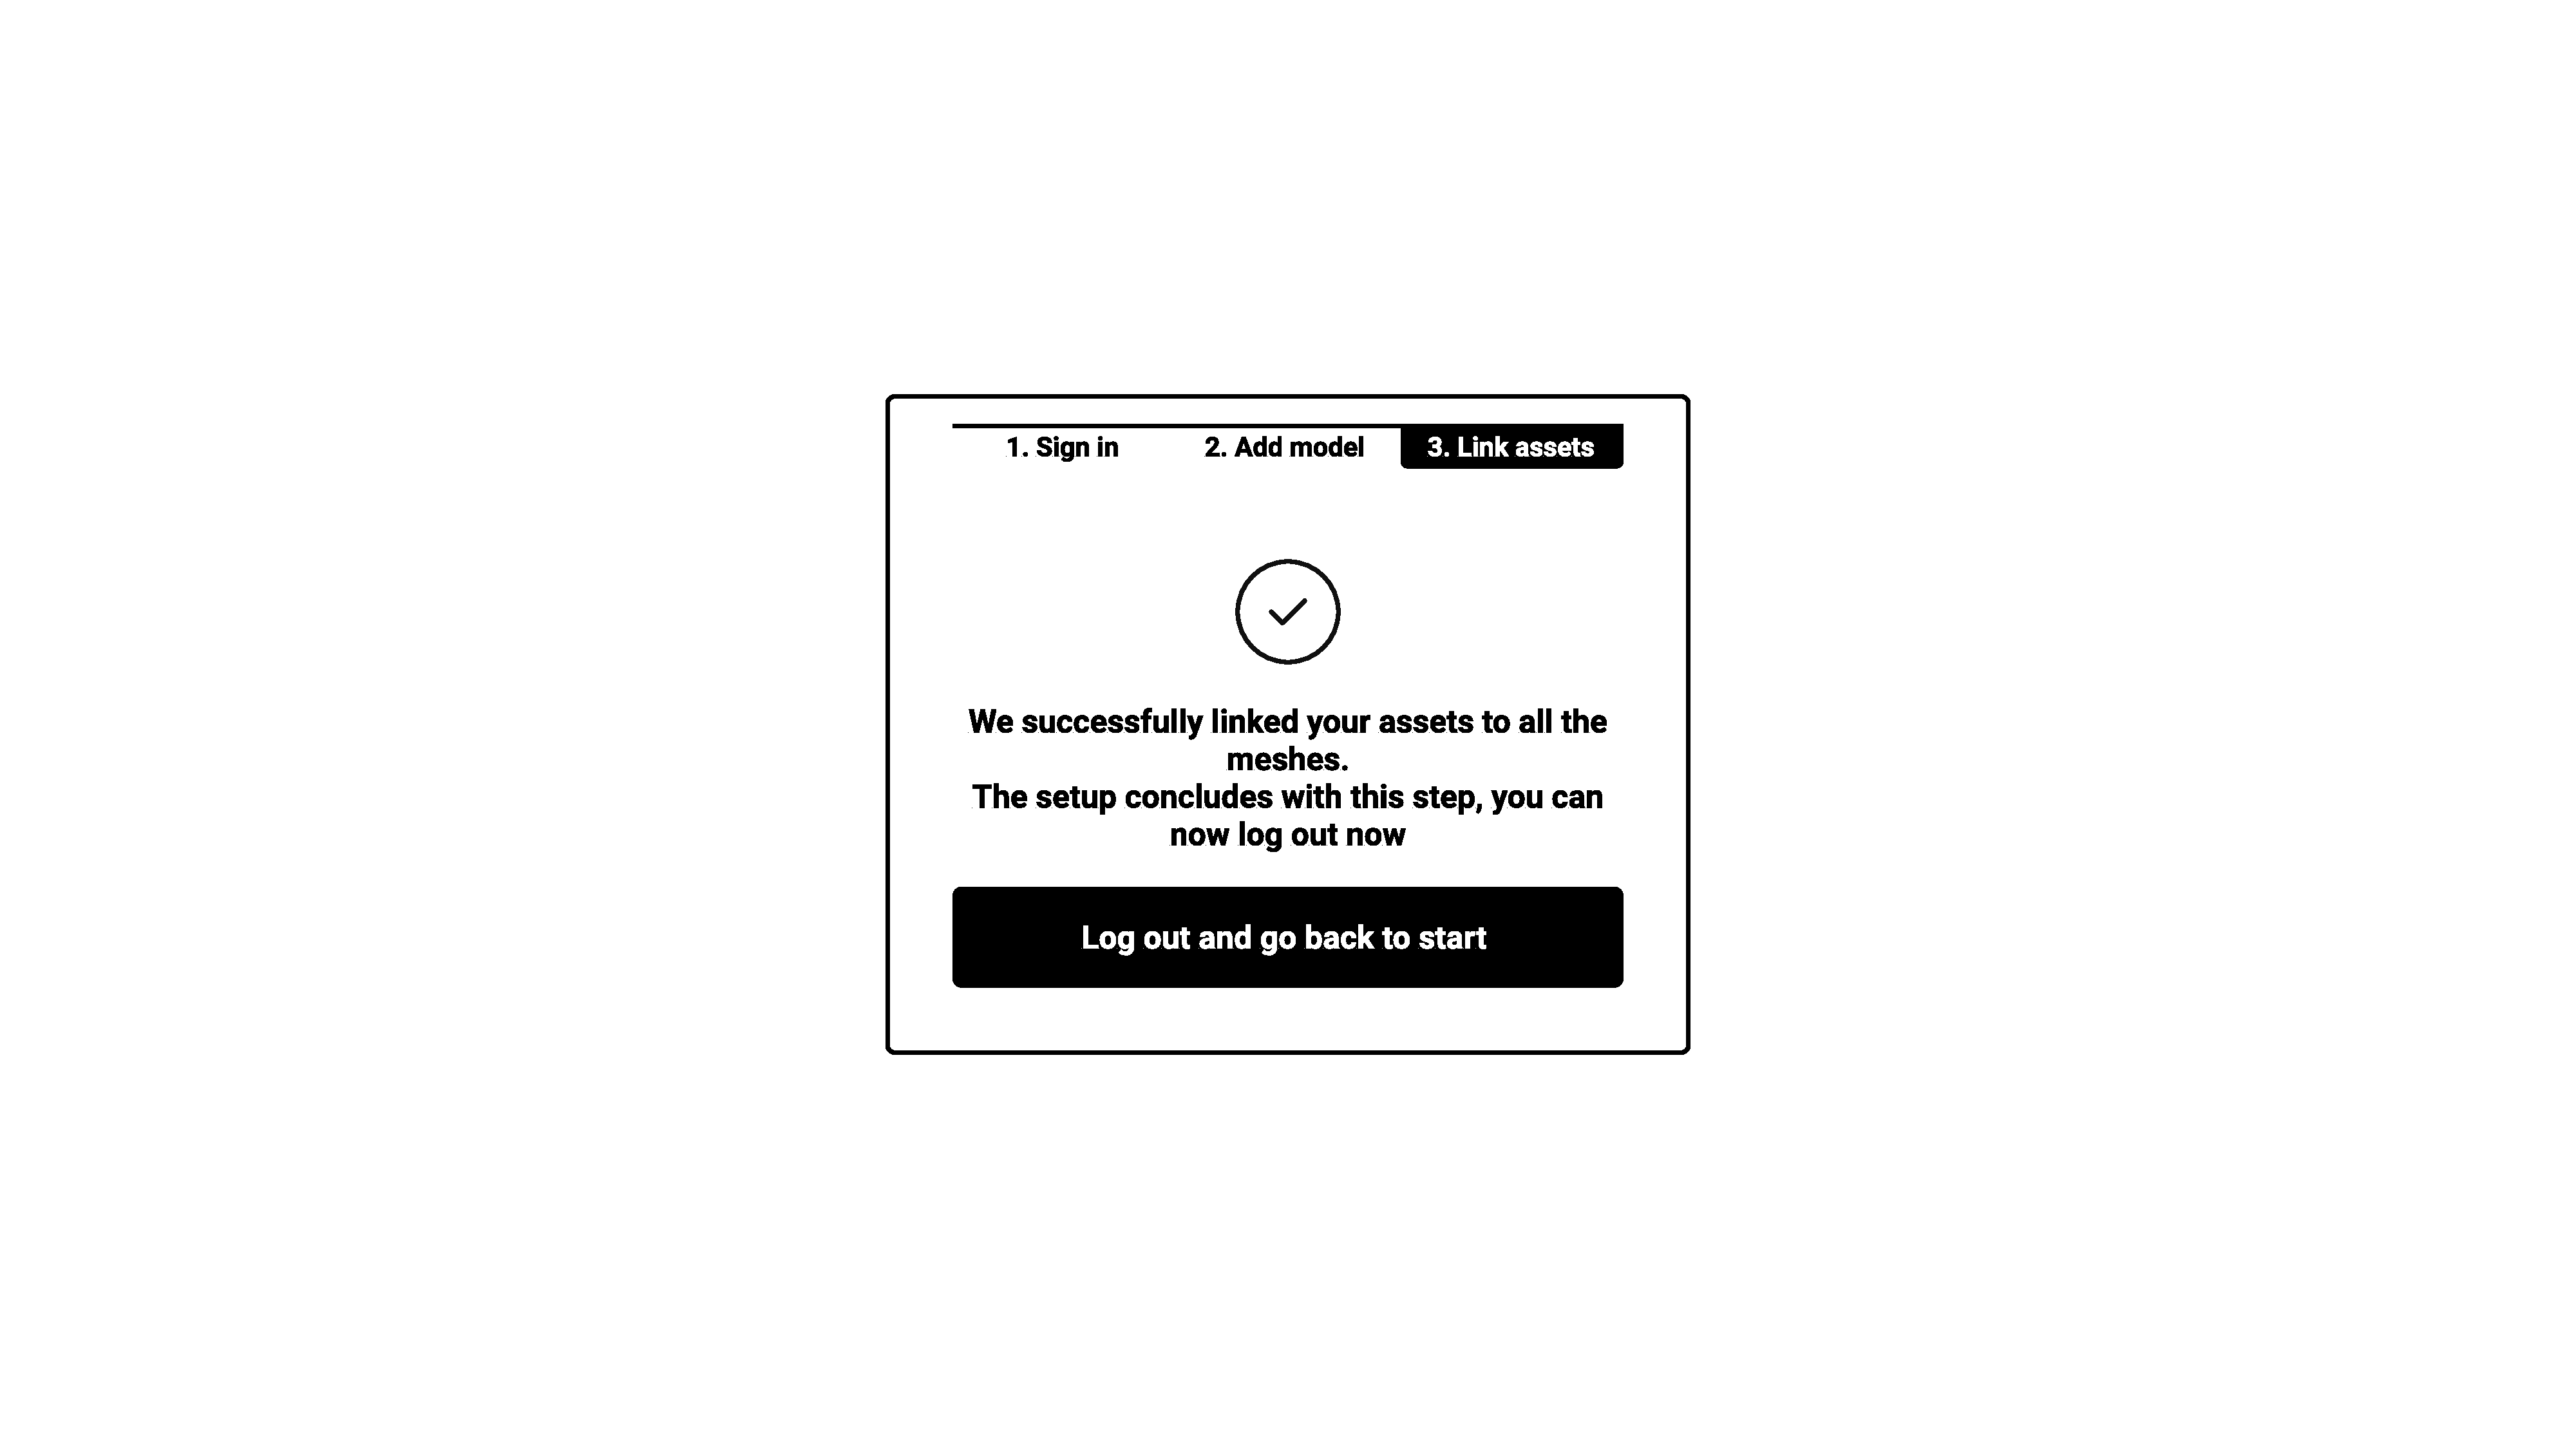
\includegraphics[angle=270,width=0.6\textwidth]{./mockups/register/all_success.pdf}
  \caption[{Mockup einer erfolgreichen Verlinkung}]{Mockup einer erfolgreichen Verlinkung}
  \label{fig:mck-all_success}
\end{figure}
\pagebreak
\subsection{Einstellungsmenü}
\subsubsection{Modeleinstellungen}
Nachfolgend ist ein Design für die Modeleinstellungsseite. Hier kann der OSE Verantwortlicher den Namen und die Beschreibung des Models ändern.
\begin{figure}[H]
  \centering
  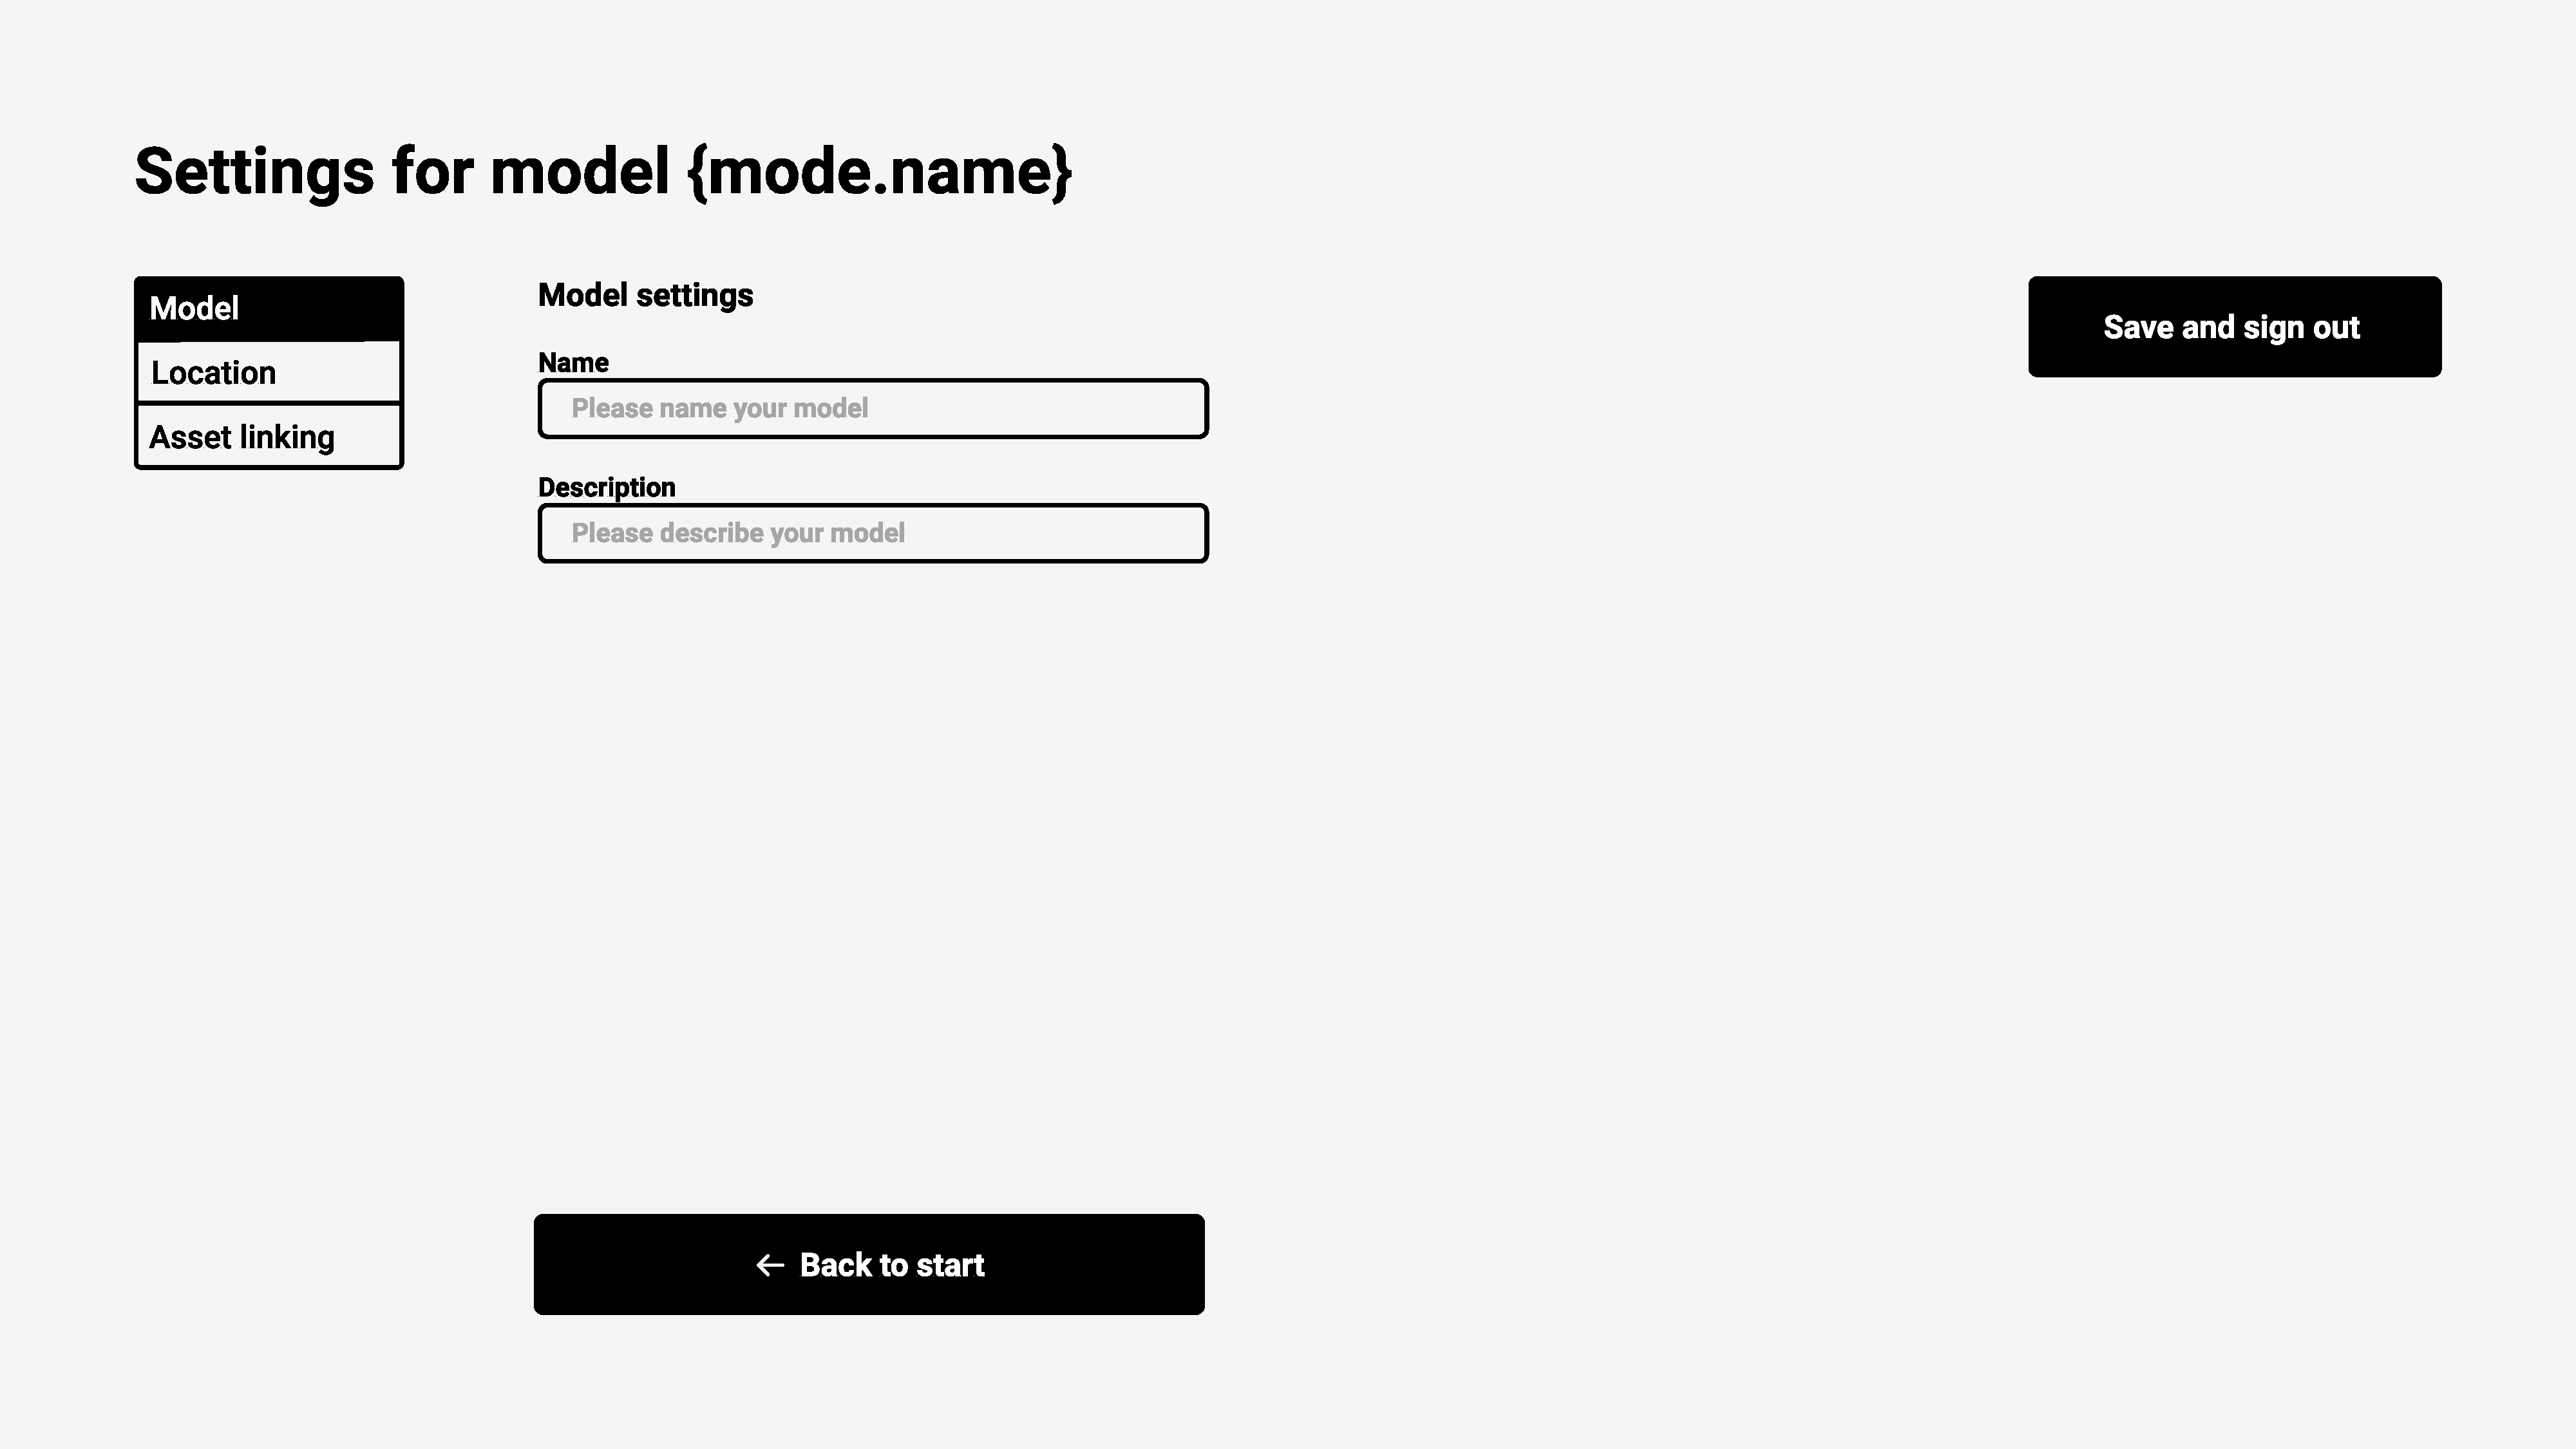
\includegraphics[angle=270,width=0.6\textwidth]{./mockups/settings/Model.pdf}
  \caption[{Mockup des Modeleinstellungsmenü}]{Mockup des Modeleinstellungsmenü}
  \label{fig:mck-model}
\end{figure}
\pagebreak
\subsubsection{Standorteinstellungen}
Dies ist das Design für die Standortseinstellungsseite. Hier kann der Standort im nachhinein verändert werden.
\begin{figure}[H]
  \centering
  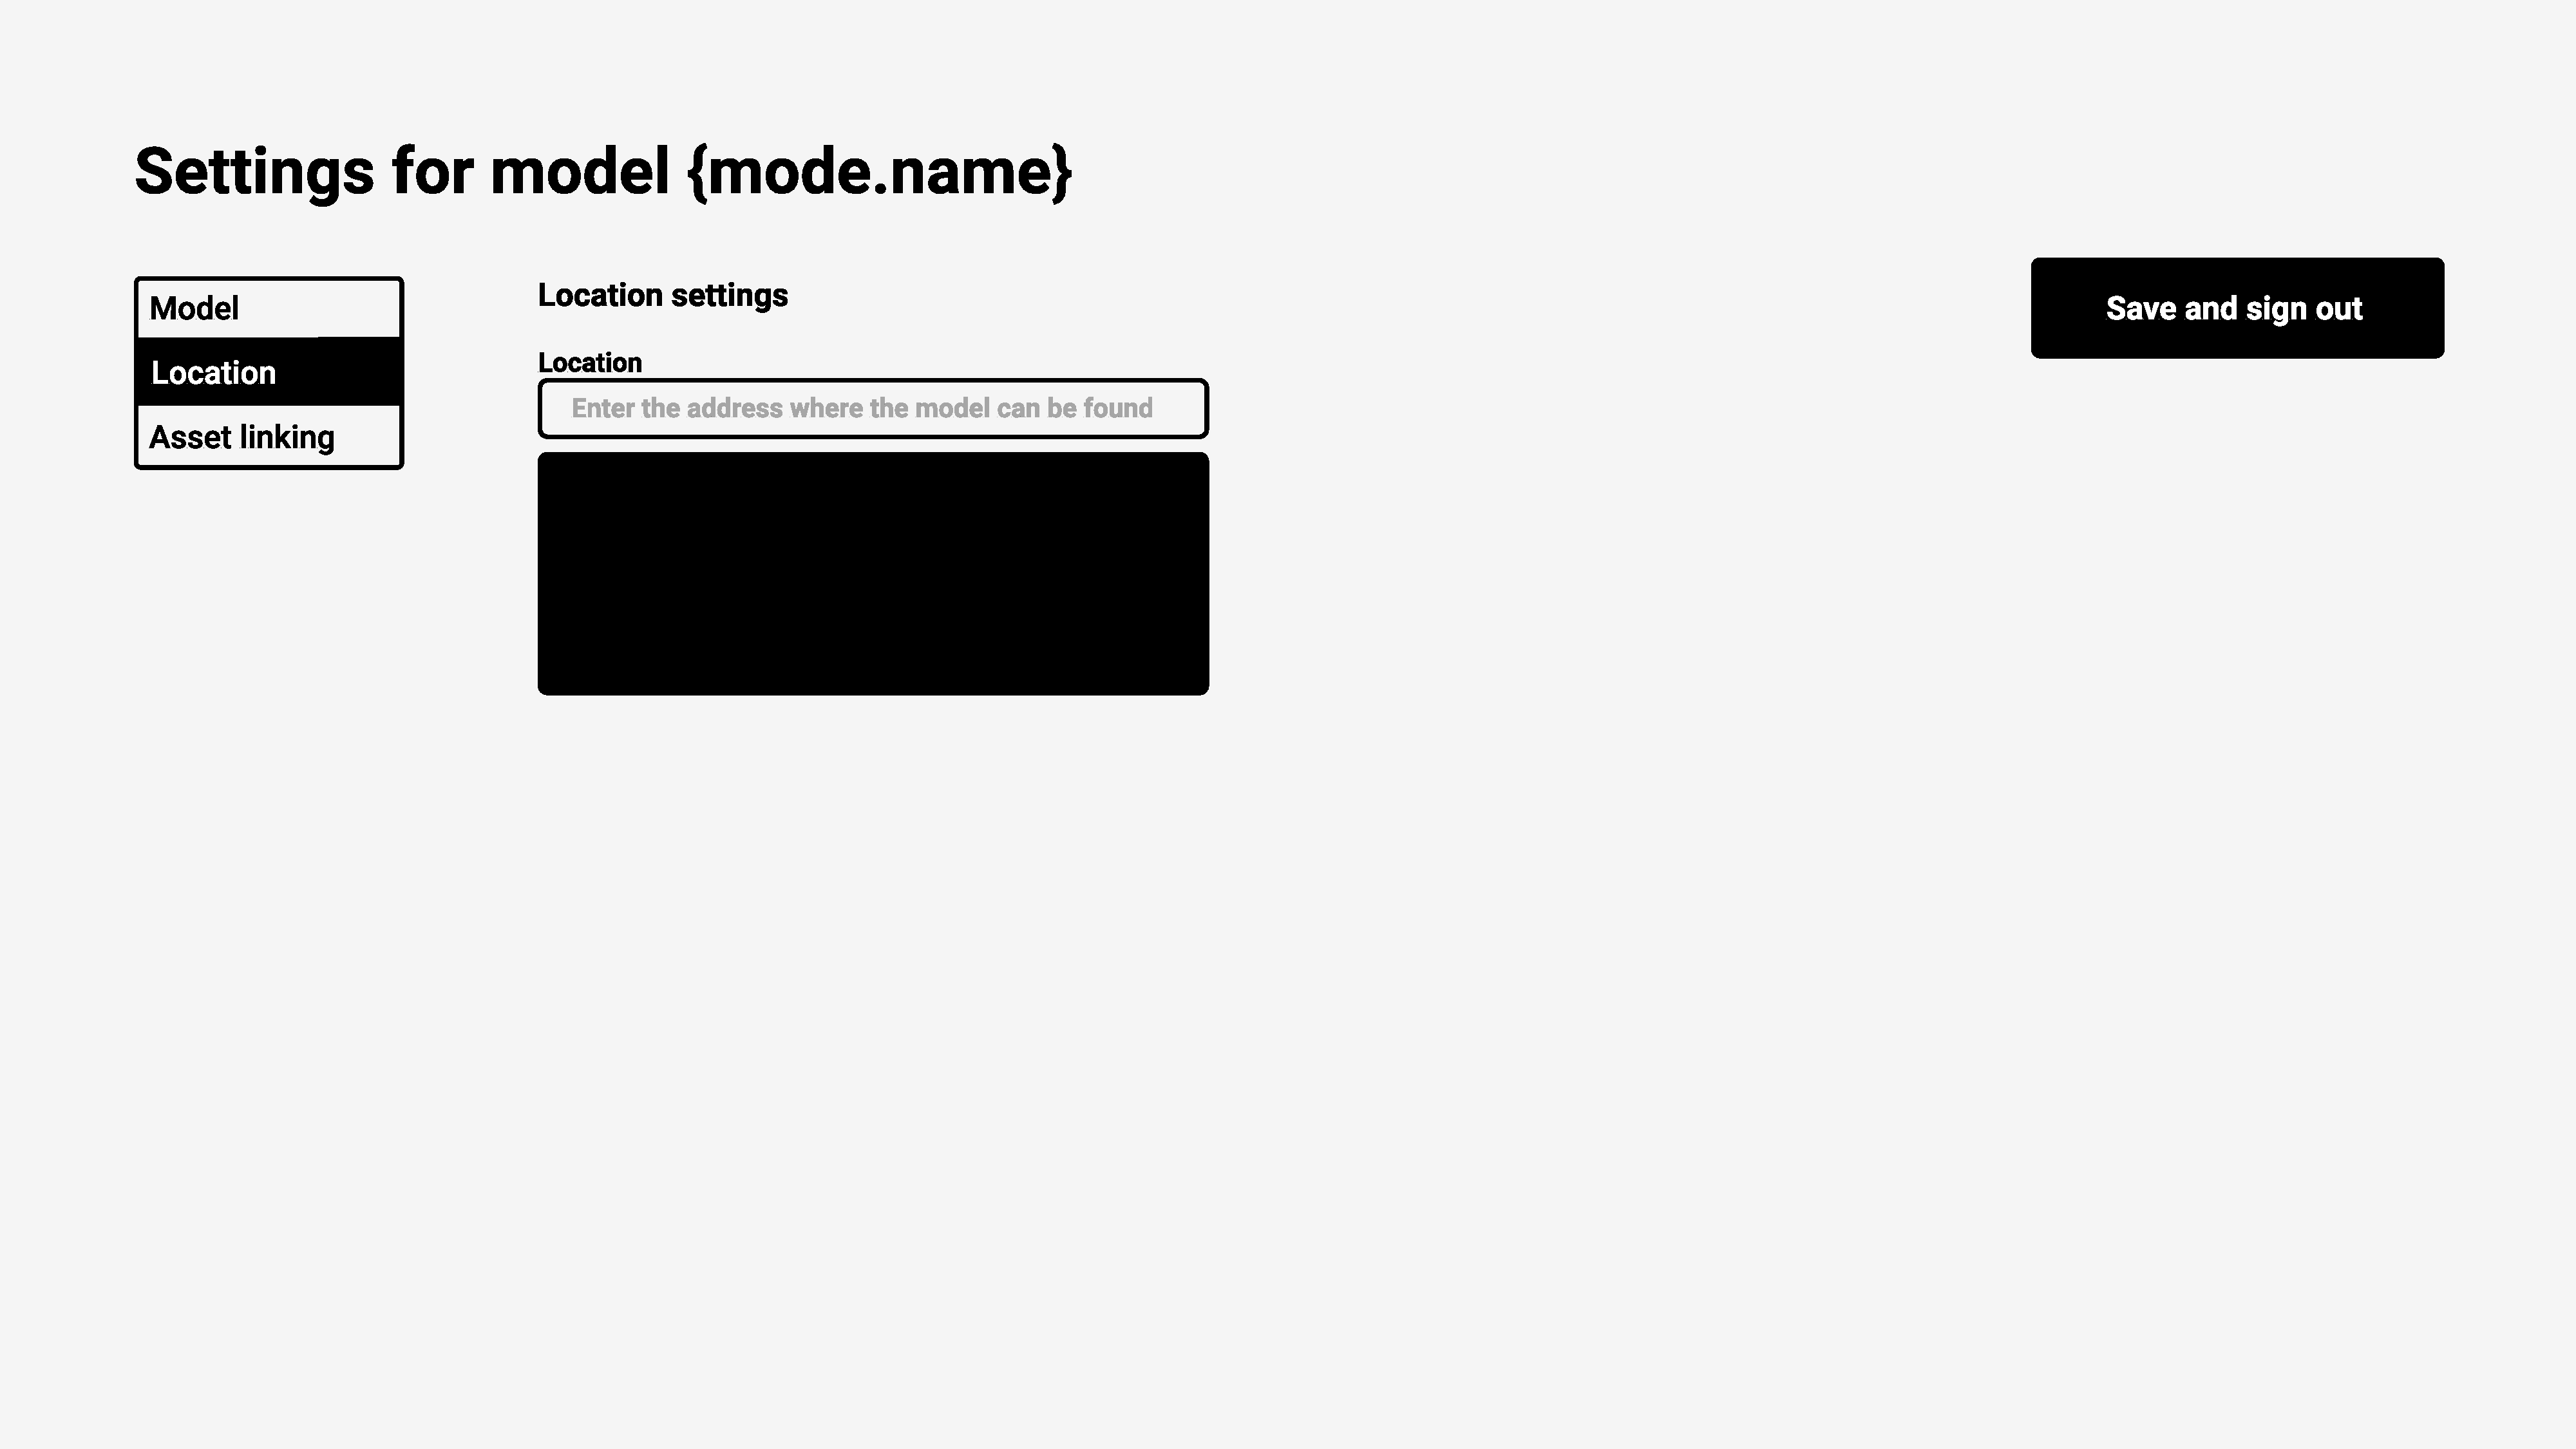
\includegraphics[angle=270,width=0.6\textwidth]{./mockups/settings/Model-1.pdf}
  \caption[{Mockup des Standorteinstellungsmenü}]{Mockup des Standorteinstellungsmenü}
  \label{fig:mck-model_1}
\end{figure}
\pagebreak
\subsubsection{Verlinkungseinstellungen}
Nachfolgend ist ein Design für die Verlinkungseinstellungsseite. Hier kann der OSE Verantwortlicher Verlinkung des Models ändern.
\begin{figure}[H]
  \centering
  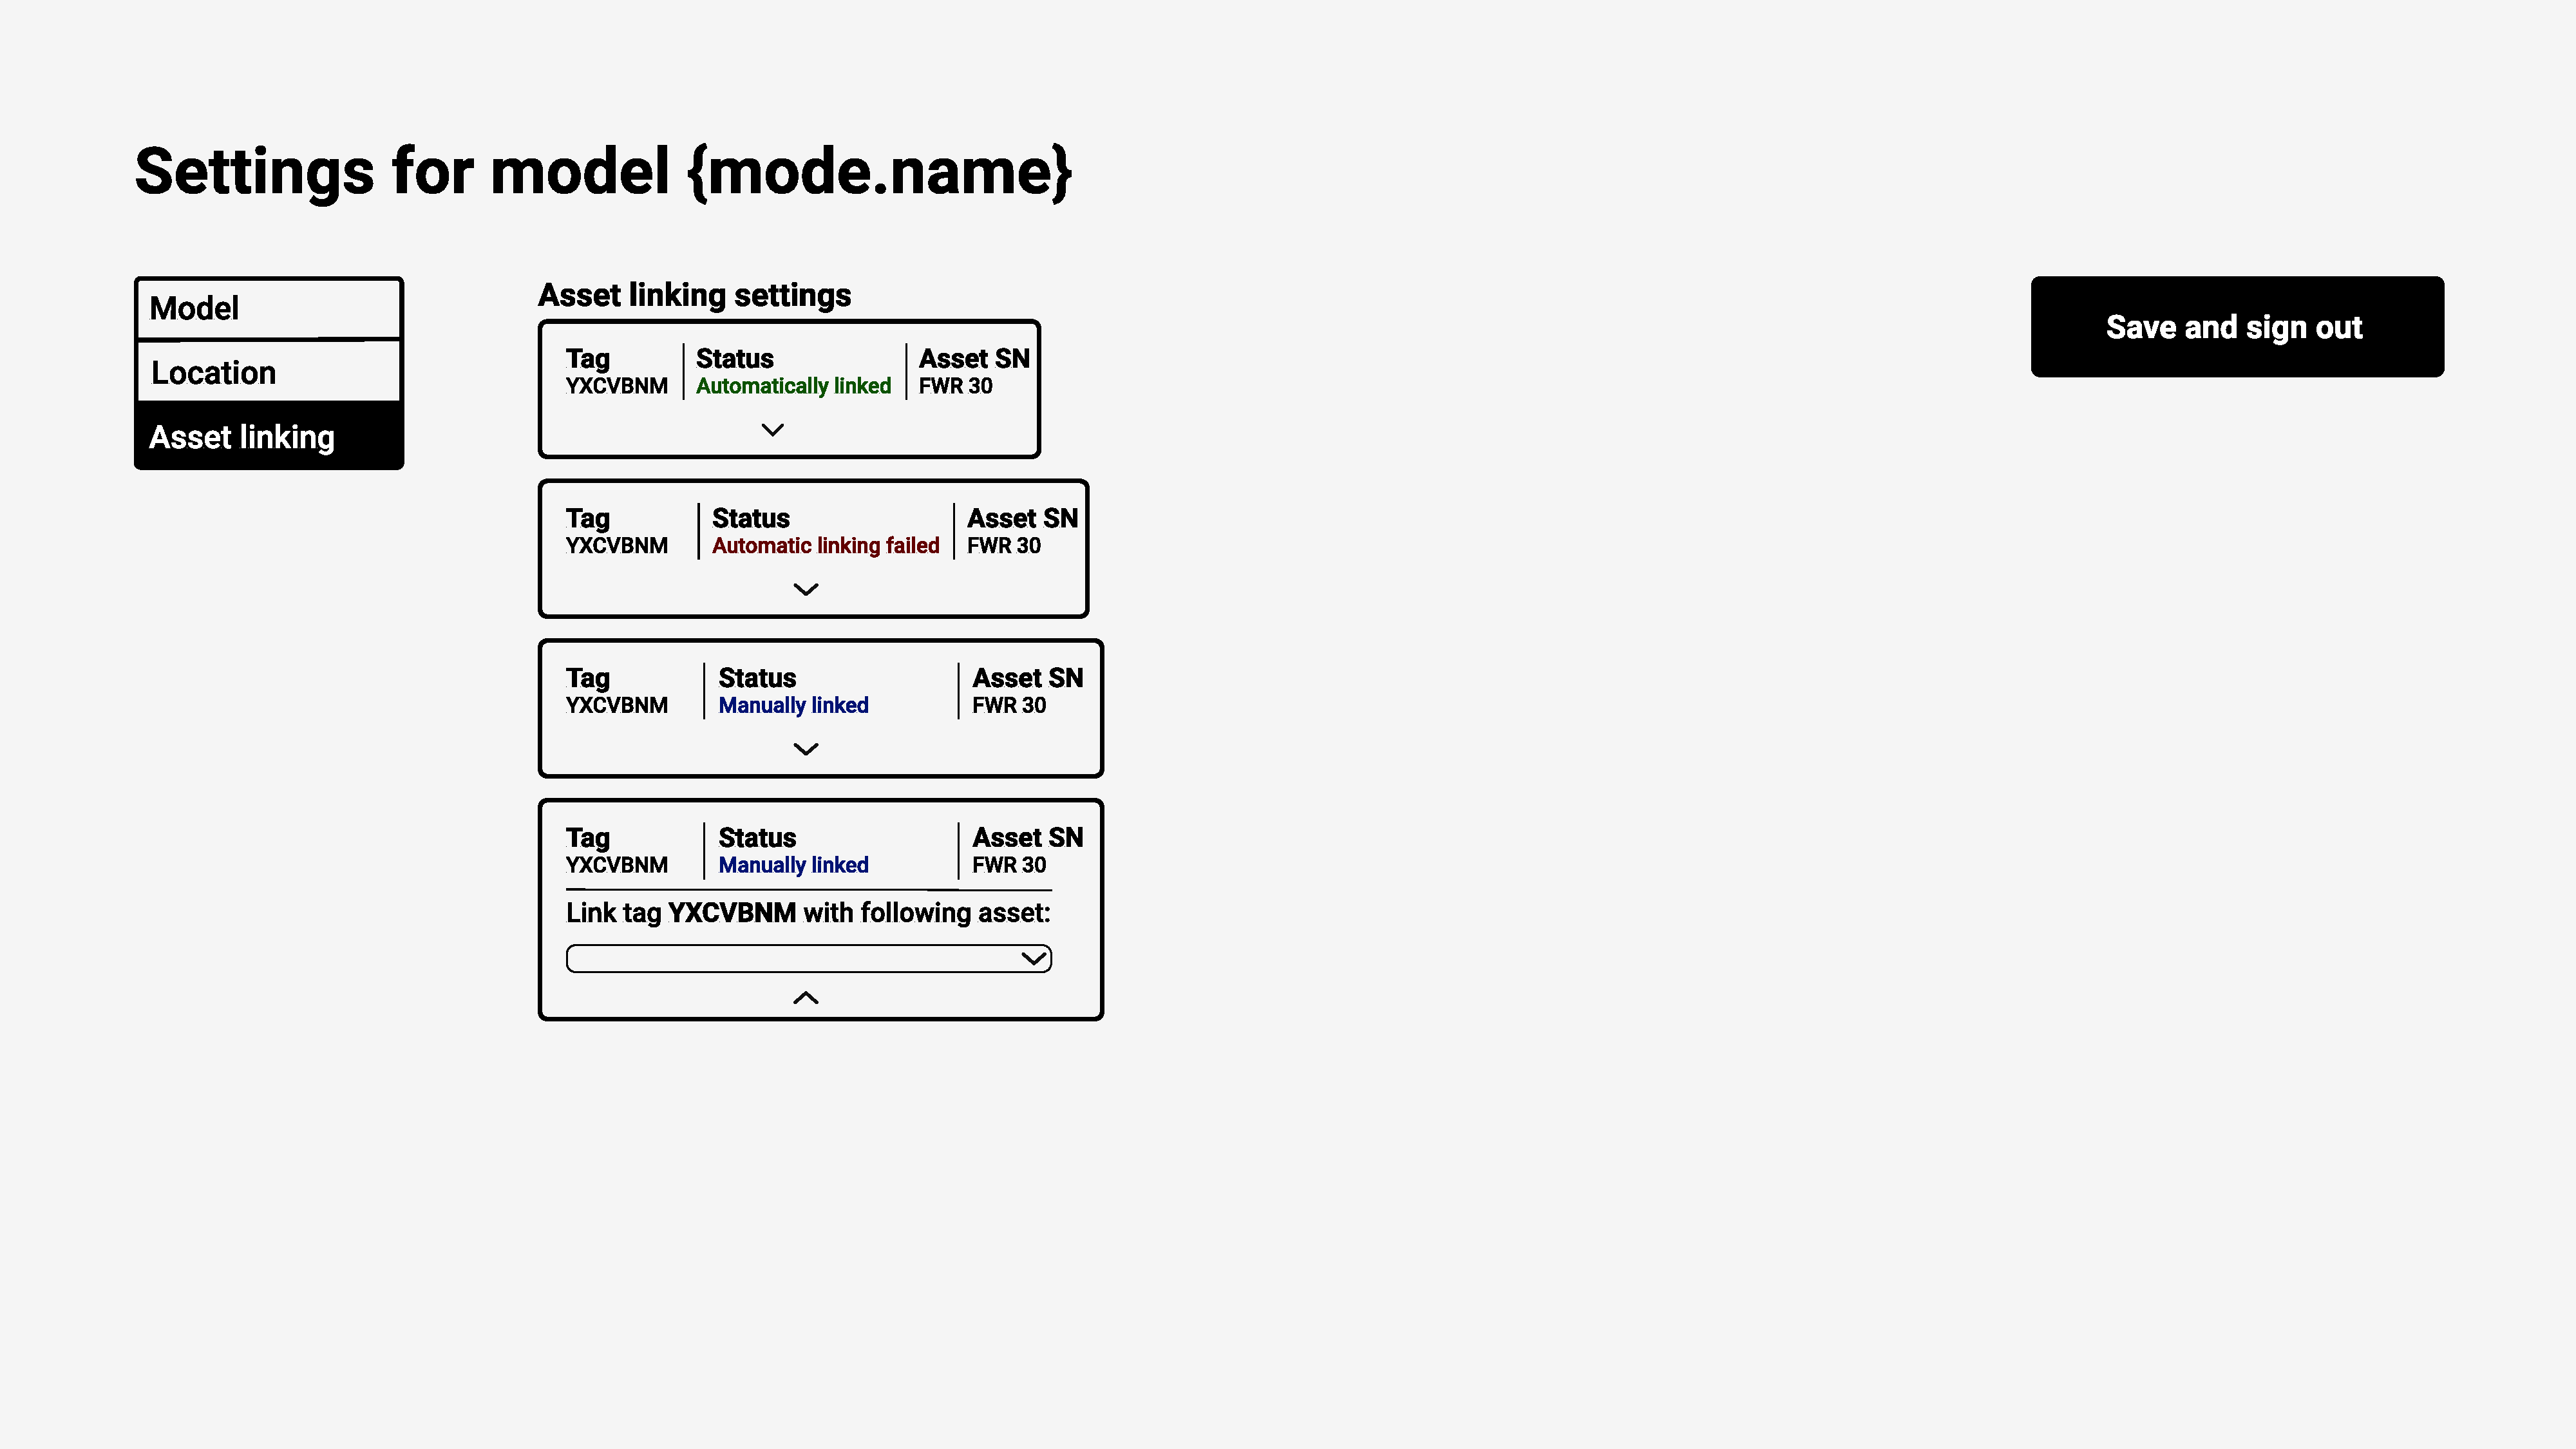
\includegraphics[angle=270,width=0.6\textwidth]{./mockups/settings/Model-2.pdf}
  \caption[{Mockup des Verlinkungseinstellungsmenü}]{Mockup des Verlinkungseinstellungsmenü}
  \label{fig:mck-model_2}
\end{figure}
\section{Testkonzept}
Damit sich bei der Abnahme des Projektes sicher gegangen werden kann, dass alles wie gewünscht funktioniert, wird ein Testkonzept erarbeitet. Dieses soll sich auf die bereits erstellten User-Stories stützen und so alle Anforderungen der Anspruchsgruppen abdecken. Nach der Implementierungsphase wird dieses Konzept befolgt und differenzen dokumentiert.
\newline
Einzelne Test-Cases werden wie folgt benannt:
\begin{table}[H]
  \begin{tabularx}{\textwidth}{l l X}\hline \\
  \textbf{Segment} & \textbf{Abkürzung} & \textbf{Beschreibung} \\ \\\hline \\
  1 & TC & Abkürzung für Test Case \\
  2 & - & Trennzeichen \\
  3 & 01 & Fortlaufende Kennzahl \\
  \\\hline
  \end{tabularx}
\end{table}
\subsection{Fehlerklassen}
Damit Testergebnisse nach der Prüfung priorisiert werden können, werden ihnen Fehlerklassen zugewiesen.
Fehlerklassen sind folgenderweise definiert:
\begin{table}[H]
  \begin{tabularx}{\textwidth}{l l X}\hline \\
  \textbf{Fehlerklasse} & \textbf{Beschreibung} \\ \\\hline \\
  0 & Definiertes Resultat stimmt mit dem getesteten Resultat überein \\
  1 & Definiertes Resultat weicht von dem getestet Resultat ab, beeinträchtigt die \\
    & Funktionalität allerdings nicht \\
  2 & Definiertes Resultat weicht von dem getestet Resultat ab und beeinträchtigt \\
    & die Funktionalität \\
  3 & Definiertes Resultat und getestetes Resultat stimmen nicht überein \\
  \\\hline
  \end{tabularx}
\end{table}
\subsection{Test Case Schema}
\begin{table}[H]
  \begin{tabularx}{\textwidth}{l l X}\hline \\
  \textbf{Segment} & \textbf{Beschreibung} \\ \\\hline \\
  Name & Name des Testes, gemäss des Namenskonzeptes \\
  Tester & Name der Person, die den Test durchgeführt hat \\
  Erwartetes Resultat & Vom Nutzer gewünschtes Resultat \\
  Effektives Resultat & Eingetroffenes Resultat \\
  Szenario & In Schritten definiertes Testszenario \\
  Fehlerklasse & Zugewiesene Fehlerklasse nach der Überprüfung \\
  Weiteres Vorgehen & Vorgehensbeschreibung, sollte die Fehlerklasse nicht 0 sein \\
  Status & Zeigt, ob der Test Case geprüft wurde \\
  \\\hline
  \end{tabularx}
\end{table}
\subsection{User-Stories Abdeckung}
\begin{table}[H]
  \begin{tabularx}{\textwidth}{l X l}\hline \\
  \textbf{Test-Case} & \textbf{Beschreibung} & \textbf{Betroffene User-Story} \\\hline \\
  TC-01 & Login möglich und sicher -> OAuth2konzept befolgt & US-01 \\
  TC-02 & Fehlermeldung Login & US-01 \\
  TC-03 & Automatische verlinkung Assets & US-02 \\
  TC-04 & Konfigurationsmenü aufrufbar & US-03 \\
  TC-05 & Verlinkungen manuel änderbar & US-03 \\
  TC-06 & Konfigurationsmenü nur durch eingeloggten User, welcher sich in der Usergruppe befindet, aufrufbar & US-04 \\
  TC-07 & Übersicht aller Standorte & US-06 \\
  TC-08 & Standort änderbar & US-06 \\
  \\\hline
  \end{tabularx}
\end{table}
\pagebreak
\subsection{Test-Cases}
\subsubsection{TC-01: Login}
\begin{table}[H]
  \begin{tabularx}{\textwidth}{l X}\hline \\
  Name & TC-01 \\
  Tester & Jonas Schultheiss \\
  Erwartetes Resultat & OSE Verantwortlicher kann sich anmelden \\
  Effektives Resultat & / \\
  Fehlerklasse & / \\
  Weiteres Vorgehen & / \\
  Status & Noch nicht durchgeführt \\
  \\\hline
  \end{tabularx}
\end{table}
\begin{table}[H]
  \begin{tabularx}{\textwidth}{l X X}
  \textbf{Schritt} & \textbf{Beschreibung} & \textbf{Erwartetes Resultat}\\ \\\hline \\
  0 & Benutzer befindet sich auf der Startseite & / \\
  1 & Benutzer klickt den Knopf "Sign in with Netilion" an & Client des Benutzers wird an Netilion ID weitergeleited \\
  2 & Benutzer gibt seine Daten an und loggt sich ein & Client des Benutzers wird zurück an das OSE-Dashboard geleited \\
  3A & Benutzer nicht registriert & Benutzer wird zur Registration weitergeleited \\
  3B & Benutzer registriert & Benutzer wird zum Konfigurationsmenü weitergeleited \\
  \\\hline
  \end{tabularx}
\end{table}
\pagebreak
\subsection{Test-Cases}
\subsubsection{TC-02: Login falsche Logindaten}
\begin{table}[H]
  \begin{tabularx}{\textwidth}{l X}\hline \\
  Name & TC-02 \\
  Tester & Jonas Schultheiss \\
  Erwartetes Resultat & Anmeldeprozess läuft schief, aber wird bei Netilion ID direkt behandelt \\
  Effektives Resultat & / \\
  Fehlerklasse & / \\
  Weiteres Vorgehen & / \\
  Status & Noch nicht durchgeführt \\
  \\\hline
  \end{tabularx}
\end{table}
\begin{table}[H]
  \begin{tabularx}{\textwidth}{l X X}
  \textbf{Schritt} & \textbf{Beschreibung} & \textbf{Erwartetes Resultat}\\ \\\hline \\
  0 & Benutzer befindet sich auf der Startseite & / \\
  1 & Benutzer klickt den Knopf "Sign in with Netilion" an & Client des Benutzers wird an Netilion ID weitergeleited \\
  2 & Benutzer gibt seine Daten an und probiert sich anzumelden & Netilion ID zeigt Fehlermeldung an \\
  \\\hline
  \end{tabularx}
\end{table}
\pagebreak
\subsubsection{TC-03: Login mit unberechtigtem Account}
\begin{table}[H]
  \begin{tabularx}{\textwidth}{l X}\hline \\
  Name & TC-03 \\
  Tester & Jonas Schultheiss \\
  Erwartetes Resultat & Anmeldeprozess funktioniert und Bentzer erhält passende Fehlermeldung \\
  Effektives Resultat & / \\
  Fehlerklasse & / \\
  Weiteres Vorgehen & / \\
  Status & Noch nicht durchgeführt \\
  \\\hline
  \end{tabularx}
\end{table}
\begin{table}[H]
  \begin{tabularx}{\textwidth}{l X X}
  \textbf{Schritt} & \textbf{Beschreibung} & \textbf{Erwartetes Resultat}\\ \\\hline \\
  0 & Benutzer befindet sich auf der Startseite & / \\
  1 & Benutzer klickt den Knopf "Sign in with Netilion" an & Client des Benutzers wird an Netilion ID weitergeleited \\
  2 & Benutzer gibt seine Daten an und meldet sich an & Client des Benutzers wird zurück an das OSE-Dashboard geleited, wo eine passende Fehlermeldung angezeigt wird \\
  \\\hline
  \end{tabularx}
\end{table}
\pagebreak
\subsubsection{TC-04: Automatische Verlinkung der Assets}
Dieser Test-Case wird zusätzlich mit automatisierten Tests abgedeckt.
\begin{table}[H]
  \begin{tabularx}{\textwidth}{l X}\hline \\
  Name & TC-04 \\
  Tester & Jonas Schultheiss \\
  Erwartetes Resultat & Assets und Meshes werden automatisch verlinkt \\
  Effektives Resultat & / \\
  Fehlerklasse & / \\
  Weiteres Vorgehen & / \\
  Status & Noch nicht durchgeführt \\
  \\\hline
  \end{tabularx}
\end{table}
\begin{table}[H]
  \begin{tabularx}{\textwidth}{l X X}
  \textbf{Schritt} & \textbf{Beschreibung} & \textbf{Erwartetes Resultat}\\ \\\hline \\
  0 & Noch nicht registrierter Benutzer hat sich bereits angemeldet und befindet sich auf dem zweiten Tab der Registration & / \\
  1 & Benutzer geht zum nächsten Tab & Client zeigt an, dass die Verlinkung im Gange ist und Backend verlinkt die Entitäten \\
  2A & Alle Assets verlinkt & Benutzer wird benachrichtigt und kann sich ausloggen \\
  2A & Nicht alle Assets verlinkt & Benutzer wird benachrichtigt und kann zum Konfigurationsmenü fortfahren \\
  \\\hline
  \end{tabularx}
\end{table}
\pagebreak
\subsubsection{TC-05: Konfigurationsmenü aufrufbar}
\begin{table}[H]
  \begin{tabularx}{\textwidth}{l X}\hline \\
  Name & TC-05 \\
  Tester & Jonas Schultheiss \\
  Erwartetes Resultat & Konfigurationsmenü ist aufrufbar \\
  Effektives Resultat & / \\
  Fehlerklasse & / \\
  Weiteres Vorgehen & / \\
  Status & Noch nicht durchgeführt \\
  \\\hline
  \end{tabularx}
\end{table}
\begin{table}[H]
  \begin{tabularx}{\textwidth}{l X X}
  \textbf{Schritt} & \textbf{Beschreibung} & \textbf{Erwartetes Resultat}\\ \\\hline \\
  0 & Bereits registrierter Benutzer befindet sich auf der Startseite  & / \\
  1 & Benutzer meldet sich an & Client wird zum Konfigurationsmenü weitergeleited \\
  \\\hline
  \end{tabularx}
\end{table}
\begin{table}[H]
  \begin{tabularx}{\textwidth}{l X X}
  \textbf{Schritt} & \textbf{Beschreibung} & \textbf{Erwartetes Resultat}\\ \\\hline \\
  0 & Noch nicht registrierter Benutzer befindet sich auf der Startseite  & / \\
  1 & Benutzer meldet sich an & Client wird zur Registration weitergeleited \\
  1 & Benutzer registriert sich & Client wird zum Konfigurationsmenü weitergeleited \\
  \\\hline
  \end{tabularx}
\end{table}
\pagebreak
\subsubsection{TC-06: Verlinkung manuell änderbar}
\begin{table}[H]
  \begin{tabularx}{\textwidth}{l X}\hline \\
  Name & TC-06 \\
  Tester & Jonas Schultheiss \\
  Erwartetes Resultat & Assets und Meshes werden manuell verlinkt \\
  Effektives Resultat & / \\
  Fehlerklasse & / \\
  Weiteres Vorgehen & / \\
  Status & Noch nicht durchgeführt \\
  \\\hline
  \end{tabularx}
\end{table}
\begin{table}[H]
  \begin{tabularx}{\textwidth}{l X X}
  \textbf{Schritt} & \textbf{Beschreibung} & \textbf{Erwartetes Resultat}\\ \\\hline \\
  0 & Bereits registrierter Benutzer befindet sich im Konfigurationsmenü im Assets Tab  & / \\
  1 & Benutzer klickt auf eine Verlinkung & Verlinkungkomponente öffnet sich \\
  2 & Benutzer klickt auf das Dropdown & Dropdown öffnet und stellt alle verfügbaren Assets dar \\
  3 & Benutzer selektiert anderes Asset & Knopf "Logout" ändert sich zu "Save and logout" \\
  4 & Benutzer klickt Knopf & Änderungen werden gespeichert, der Benutzer ausgeloggt und der Client wird an die Startseite weitergeleited \\
  \\\hline
  \end{tabularx}
\end{table}
\pagebreak
\subsubsection{TC-07: Übersicht aller Standorte}
\begin{table}[H]
  \begin{tabularx}{\textwidth}{l X}\hline \\
  Name & TC-07 \\
  Tester & Jonas Schultheiss \\
  Erwartetes Resultat & Benutzer sieht übersicht aller Standorte \\
  Effektives Resultat & / \\
  Fehlerklasse & / \\
  Weiteres Vorgehen & / \\
  Status & Noch nicht durchgeführt \\
  \\\hline
  \end{tabularx}
\end{table}
\begin{table}[H]
  \begin{tabularx}{\textwidth}{l X X}
  \textbf{Schritt} & \textbf{Beschreibung} & \textbf{Erwartetes Resultat}\\ \\\hline \\
  0 & Benutzer befindet sich auf der Startseite  & / \\
  1 & Benutzer öffnet die Augen & Benutzer sieht auf der initialen Ansicht der Startseite die Standortauswahl \\
  \\\hline
  \end{tabularx}
\end{table}
\pagebreak
\subsubsection{TC-08: Standort änderbar}
\begin{table}[H]
  \begin{tabularx}{\textwidth}{l X}\hline \\
  Name & TC-08 \\
  Tester & Jonas Schultheiss \\
  Erwartetes Resultat & Standort ist änderbar \\
  Effektives Resultat & / \\
  Fehlerklasse & / \\
  Weiteres Vorgehen & / \\
  Status & Noch nicht durchgeführt \\
  \\\hline
  \end{tabularx}
\end{table}
\begin{table}[H]
  \begin{tabularx}{\textwidth}{l X X}
  \textbf{Schritt} & \textbf{Beschreibung} & \textbf{Erwartetes Resultat}\\ \\\hline \\
  0 & Bereits registrierter Benutzer befindet sich auf der Startseite  & / \\
  1 & Benutzer meldet sich an & Benutzer wird angemeldet und zum Konfigurationsmenü weitergeleitet \\
  2 & Benutzer klickt auf den Tab "Location" & Benutzer wird zu \code{/settings/location} weitergeleitet \\
  3 & Benutzer gibt im Eingabefeld eine neue Addresse ein & Addresse wird automatisch vervollständigt \\
  4 & Benutzer klickt auf den Knopf "Save changes and logout" & Änderungen werden gespeichert, der Benutzer ausgeloggt und der Client wird an die Startseite weitergeleited \\
  \\\hline
  \end{tabularx}
\end{table}
